\chapter{Results}
\label{ch:results}

We present the results in the order of the thesis argument. On these output metrics the four unlearning
methods look alike (Section~\ref{sec:r-output}); the internal readout can, and shows that
unlearning suppresses at the output rather than erasing the representation
(Section~\ref{sec:r-suppression}); confidence at the output is not knowledge (Section~\ref{sec:r-confidence});
the internal verdict is strongly scale-dependent (Section~\ref{sec:r-scale}); the derived metric
$D_\text{mech}$ is, under the field's own meta-evaluation, the most faithful metric on Hubble-8B
(Section~\ref{sec:r-faithful}), and it is far more paraphrase-stable than the lexical metrics
(Section~\ref{sec:r-invariance}); and a comparison of the three lenses explains why the metric is built on
the logit lens (Section~\ref{sec:r-lenses}). Section~\ref{sec:r-limits} states the limitations honestly.

\section{The Output View Does Not Separate the Methods}
\label{sec:r-output}

Table~\ref{tab:infill} reports infill accuracy (chance $\approx 0.10$) for all six models at both scales.
The Perturbed model recalls the fact almost perfectly at 8B; every unlearned method drives the Unlearn
accuracy down towards the Standard never-knew floor, while (with the exception of RMU, whose retain
collapses) preserving the Keep set. At the output the four methods are essentially indistinguishable, and
all look like successful, selective unlearning. Figure~\ref{fig:infill} shows the same story visually.
No single output number reveals \emph{how} each method achieves this, or whether the knowledge is gone.

\begin{table}[t]
  \centering
  \caption[Infill accuracy at both scales]{Infill accuracy (full-prefix format, chance $\approx 0.10$). Unlearning drives Unlearn towards
  the never-knew floor while preserving Keep; the four methods look alike at the output.}
  \label{tab:infill}
  \begin{tabular}{lcccc}
    \toprule
    & \multicolumn{2}{c}{\textbf{8B}} & \multicolumn{2}{c}{\textbf{1B}} \\
    \cmidrule(lr){2-3}\cmidrule(lr){4-5}
    model & Unlearn & Keep & Unlearn & Keep \\
    \midrule
    Standard \emph{(never knew)} & 0.16 & 0.13 & 0.18 & 0.09 \\
    Perturbed \emph{(knows)}     & \textbf{1.00} & \textbf{1.00} & \textbf{0.43} & \textbf{0.58} \\
    NPO      & 0.09 & 1.00 & 0.05 & 0.80 \\
    GradDiff & 0.16 & 1.00 & 0.16 & 0.60 \\
    IDK      & 0.32 & 0.98 & 0.07 & 0.82 \\
    RMU      & 0.11 & 0.64 & 0.16 & 0.33 \\
    \bottomrule
  \end{tabular}
\end{table}

\begin{figure}[t]
  \centering
  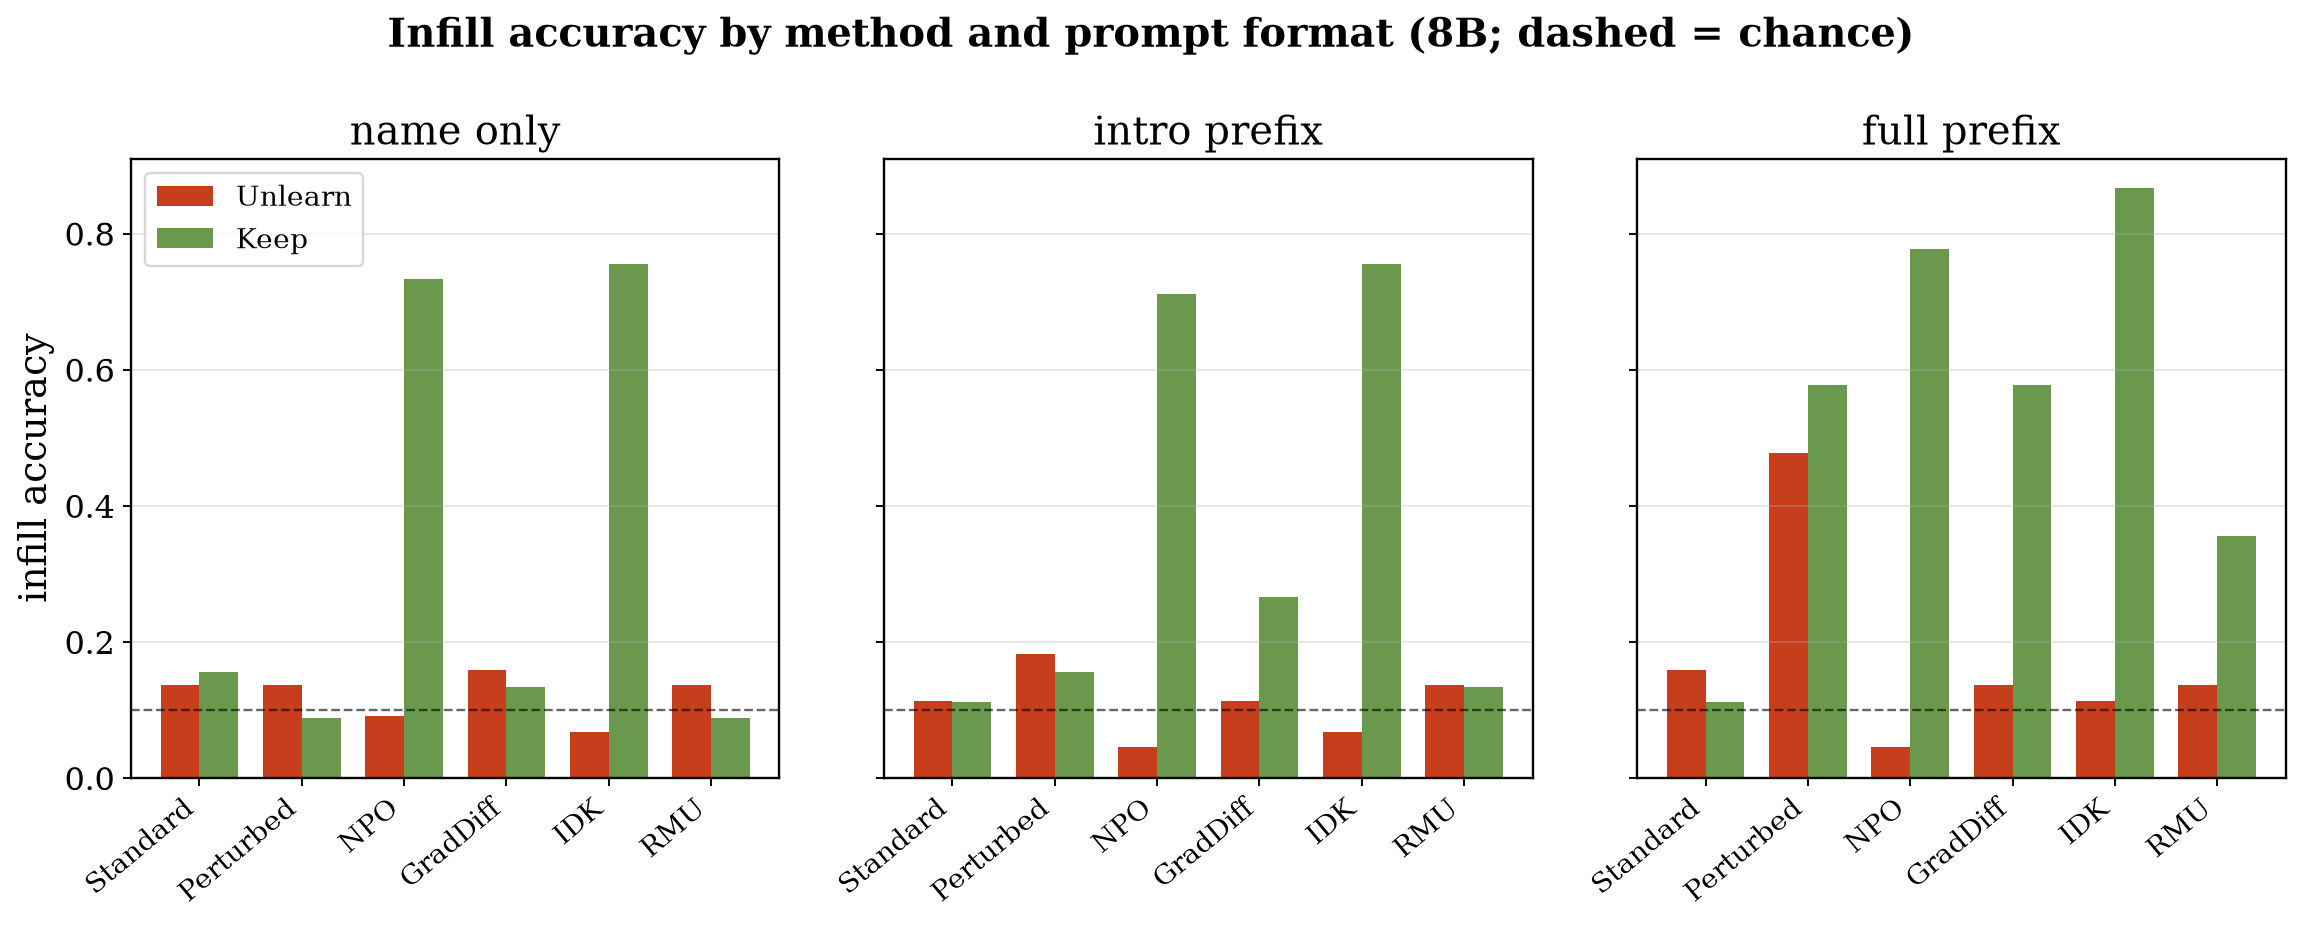
\includegraphics[width=0.85\textwidth]{infill_bars_8b}
  \caption[Infill accuracy by method (8B)]{Infill accuracy by method and prompt format (8B). Every unlearned method sits near the
  never-knew floor, and the output metrics do not tell them apart.}
  \label{fig:infill}
\end{figure}

\section{Reading the Model Layer by Layer}
\label{sec:r-suppression}

The internal readout tells a different story. Table~\ref{tab:ranks} reports the final-layer median rank of
the gold birthdate token under the corrected logit lens, and Figure~\ref{fig:logit8b} shows the full
rank-by-layer trajectories at 8B. At 8B, NPO, GradDiff, and RMU bury the fact at the output (ranks in the
thousands), but IDK does not. Its final rank of $9$ coincides with the never-knew Standard model's rank of
$9$, so at the final layer alone the two are indistinguishable. Any distinction between them must therefore
come from the full trajectory rather than the final rank, which is what the dual-anchor distance
$D_\text{mech}$ measures; Section~\ref{sec:r-faithful} and the per-fact distribution in
Section~\ref{sec:r-crossbench} report where IDK falls between the two anchors, and read its ``forgetting''
as a surface redirection to the extent that its dual-anchor distance sits above the never-knew reference. A
finer read of the mid-stack shows that NPO and GradDiff keep the token accessible in the middle layers and
only mask it late, whereas RMU buries it deepest mid-stack. One output verdict thus corresponds to different
internal mechanisms. Within the reliable mid-to-late-layer band, none of the evaluated methods consistently
matches the never-knew reference. Each keeps the gold token recoverable there, an outcome we describe as
residual internal accessibility rather than erasure.

\begin{table}[t]
  \centering
  \caption[Final-layer rank of the gold token]{Final-layer median rank of the gold token under the corrected logit lens (lower = more
  recoverable). Retain is preserved everywhere (rank $1$ to $6$); the forget signatures differ by method and
  scale.}
  \label{tab:ranks}
  \begin{tabular}{lcccc}
    \toprule
    & \multicolumn{2}{c}{\textbf{8B}} & \multicolumn{2}{c}{\textbf{1B}} \\
    \cmidrule(lr){2-3}\cmidrule(lr){4-5}
    model & forget & retain & forget & retain \\
    \midrule
    Standard \emph{(never knew)} & 9 & 10 & 10 & 11 \\
    Perturbed \emph{(knows)}     & \textbf{1} & 1 & \textbf{4} & 3 \\
    NPO      & \textbf{3{,}863} & 1 & \textbf{44{,}226} & 1 \\
    GradDiff & \textbf{9{,}191} & 1 & 8 & 3 \\
    IDK      & 9 & 1 & 16 & 1 \\
    RMU      & \textbf{2{,}693} & 2 & 8 & 6 \\
    \bottomrule
  \end{tabular}
\end{table}

\begin{figure}[t]
  \centering
  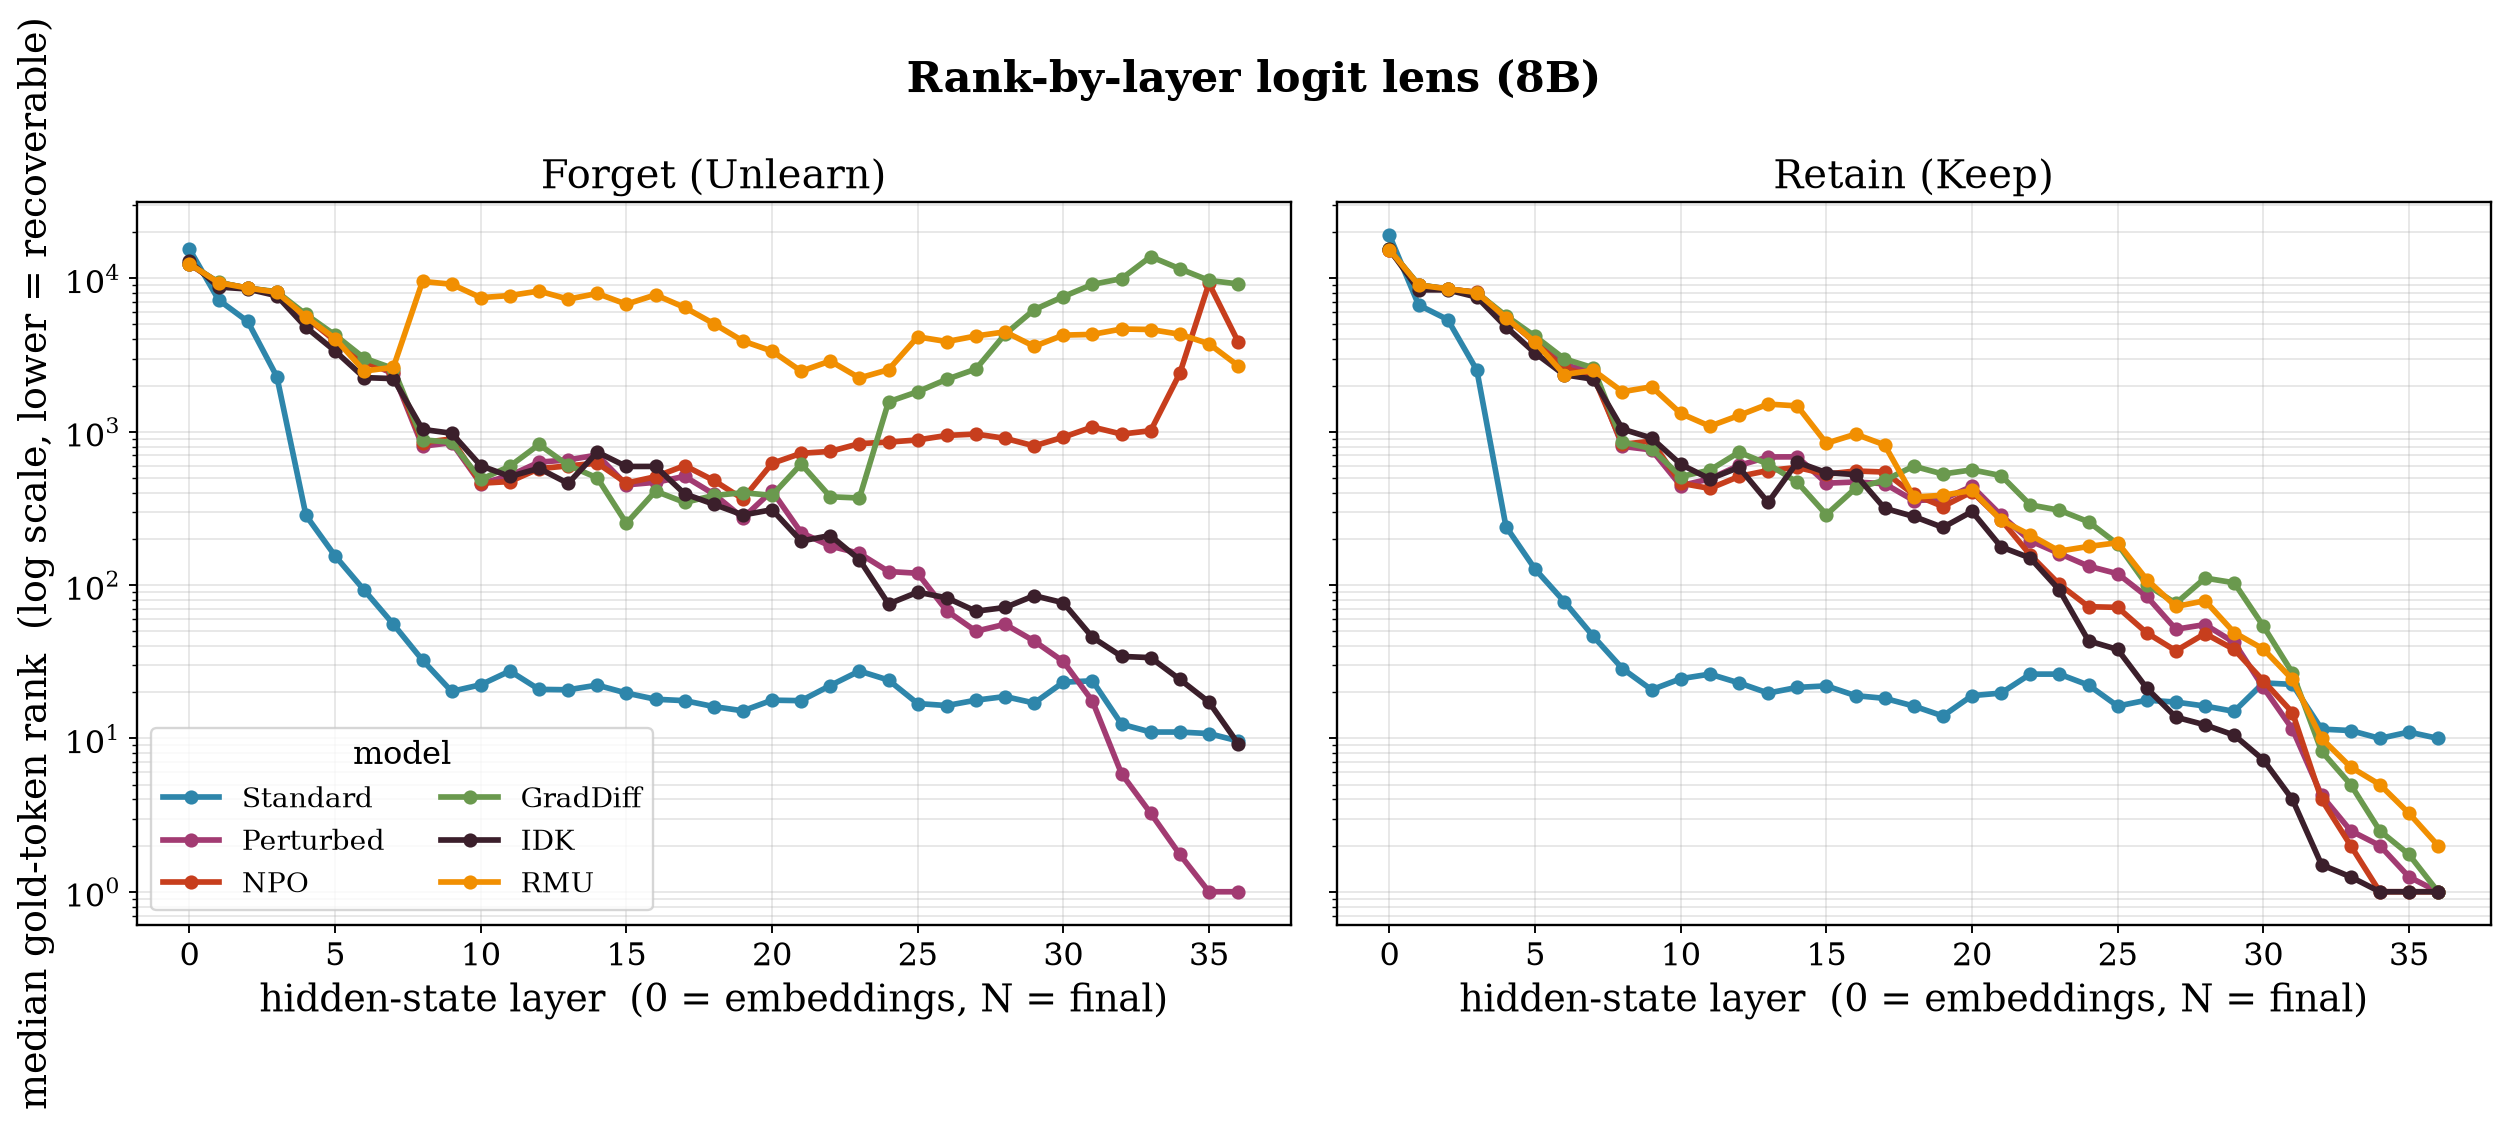
\includegraphics[width=0.92\textwidth]{logitlens_rank_median_8b}
  \caption[Rank-by-layer logit lens (8B)]{Rank-by-layer logit lens at 8B, forget (left) and retain (right). Lower is more recoverable.
  Retain is preserved for all methods; the forget trajectories separate the four mechanisms that
  Table~\ref{tab:infill} could not.}
  \label{fig:logit8b}
\end{figure}

The single-fact view in Figure~\ref{fig:lenstable} makes the suppression-versus-erasure distinction
concrete. On the same prompt, the Perturbed model's top-1 prediction climbs across layers to the correct
month at near-certain confidence, whereas the unlearned model never surfaces it and instead decodes a
meaningless token. This is consistent with output suppression while a residual internal trace persists
under the applied readout.

\begin{figure}[t]
  \centering
  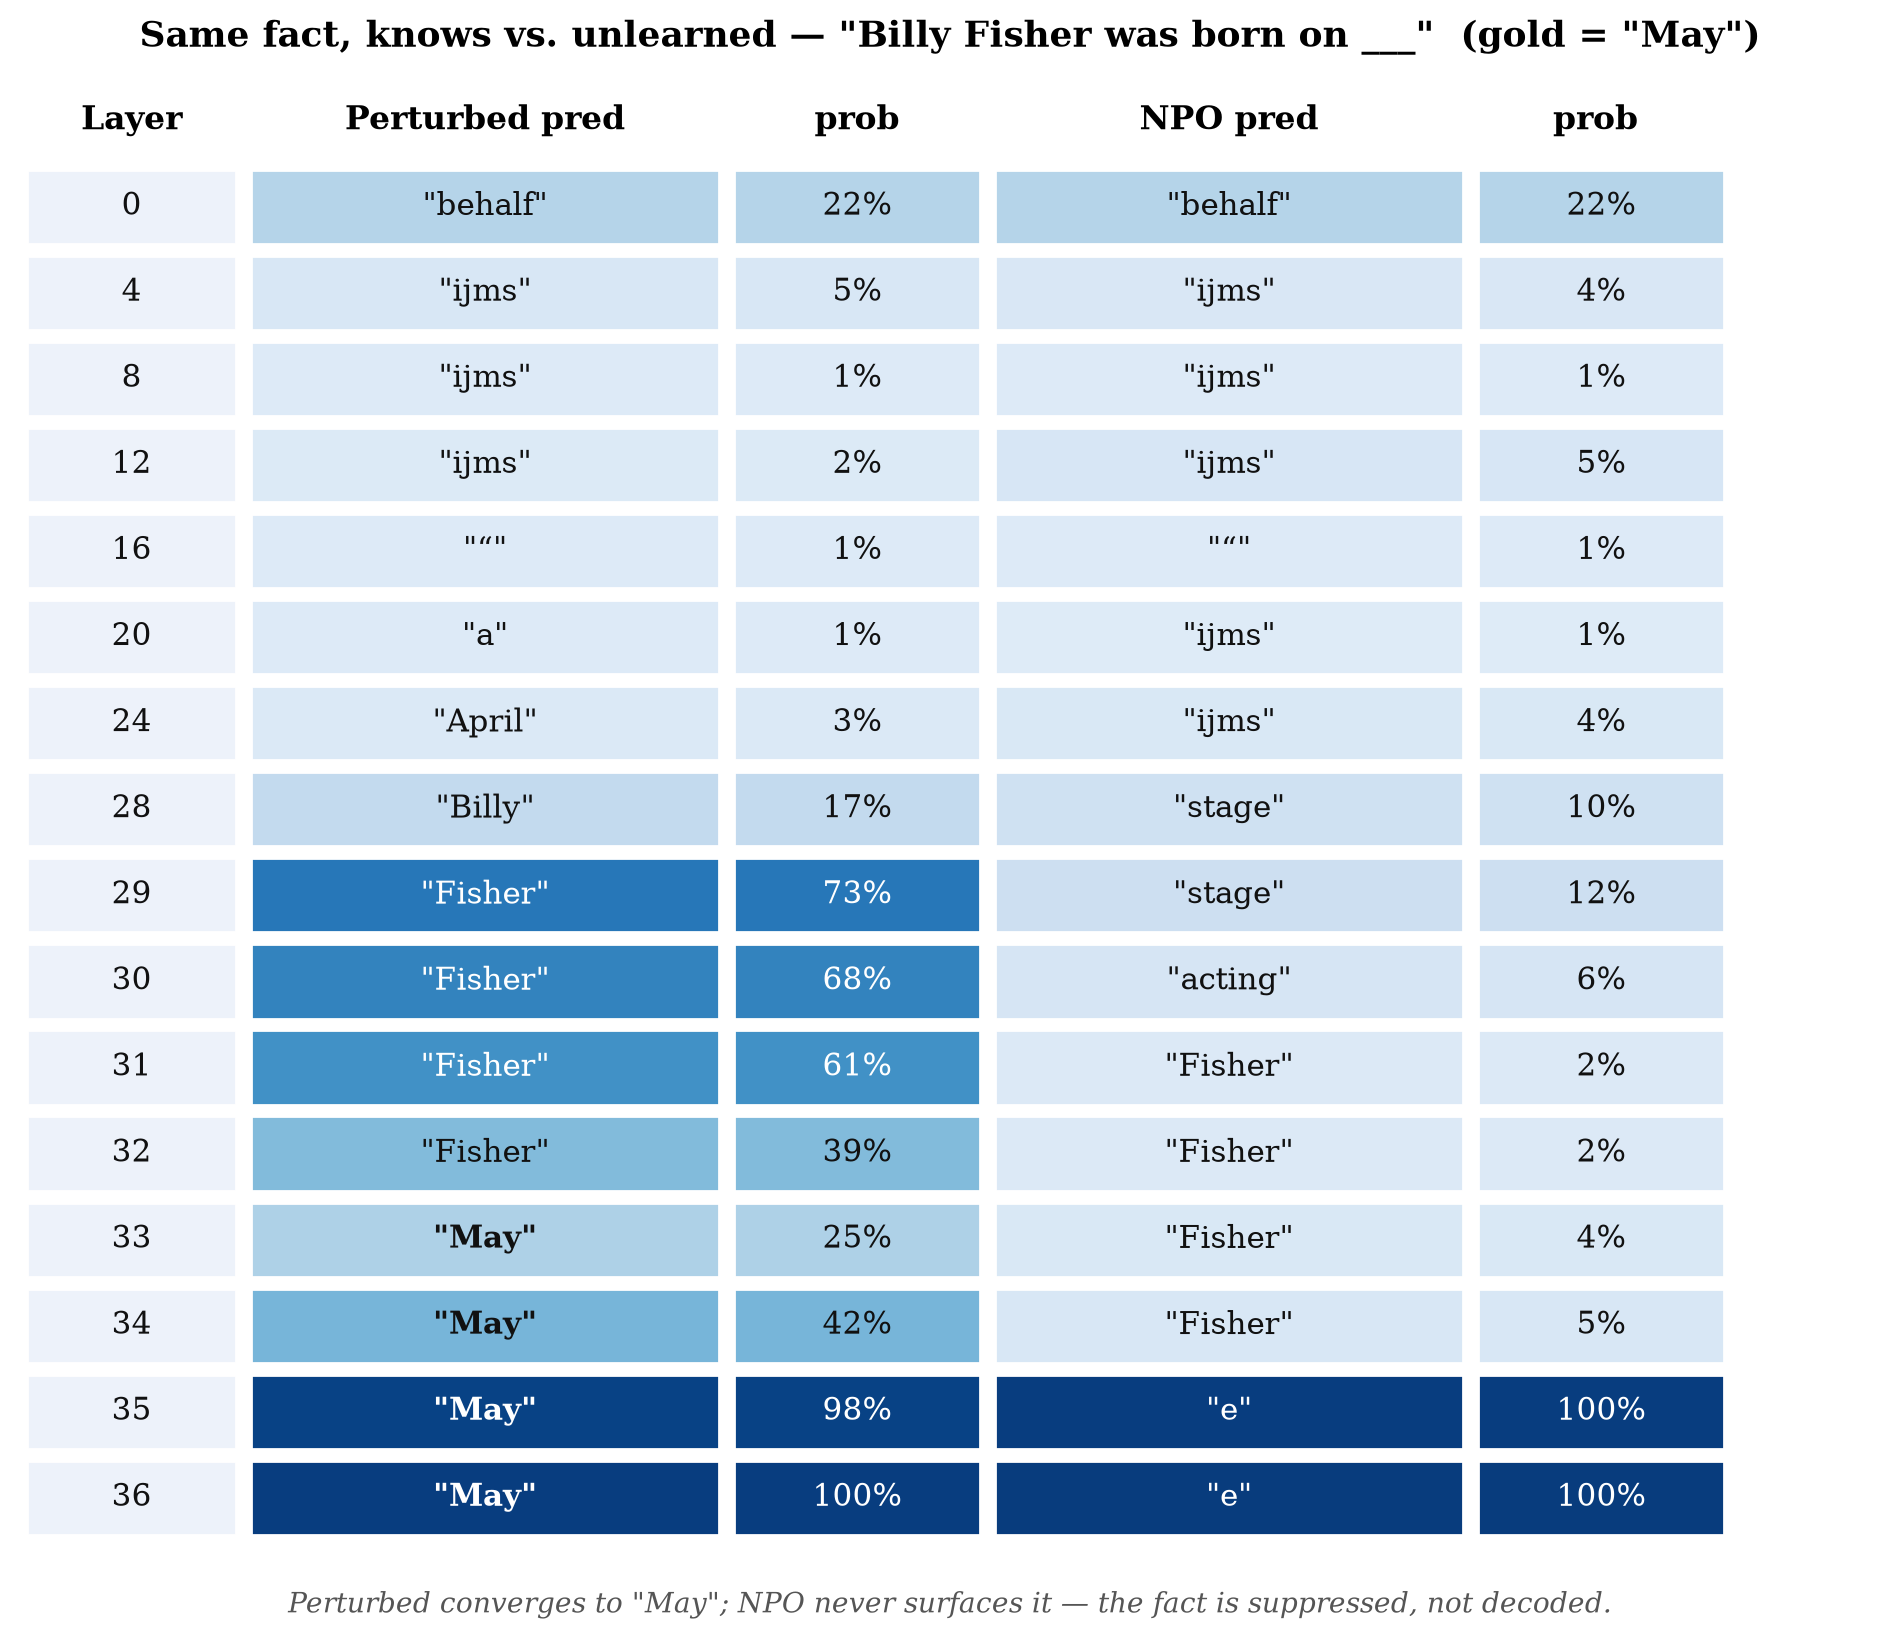
\includegraphics[width=0.9\textwidth]{lenstable_contrast_0}
  \caption[Emergence versus suppression (8B)]{Top-1 logit-lens prediction at every layer (8B), for a model that knows (left) versus an
  unlearned model on the \emph{same} fact (right). The knowing model converges to the answer; the
  unlearned model never surfaces it. Suppression, not erasure.}
  \label{fig:lenstable}
\end{figure}

\section{Confidence is not Knowledge}
\label{sec:r-confidence}

Figure~\ref{fig:confidence} lines up the final-layer prediction of all six models on the same question.
Three unlearned methods emit a \emph{wrong} token at essentially $100\%$ confidence, the same confidence
as the model that actually knows the answer. A probability- or confidence-based metric therefore cannot
separate ``confidently knows'' from ``confidently deflects''; this is the failure of output metrics made
visual, and it directly motivates a metric that reads the internal trajectory rather than the output
confidence.

\begin{figure}[t]
  \centering
  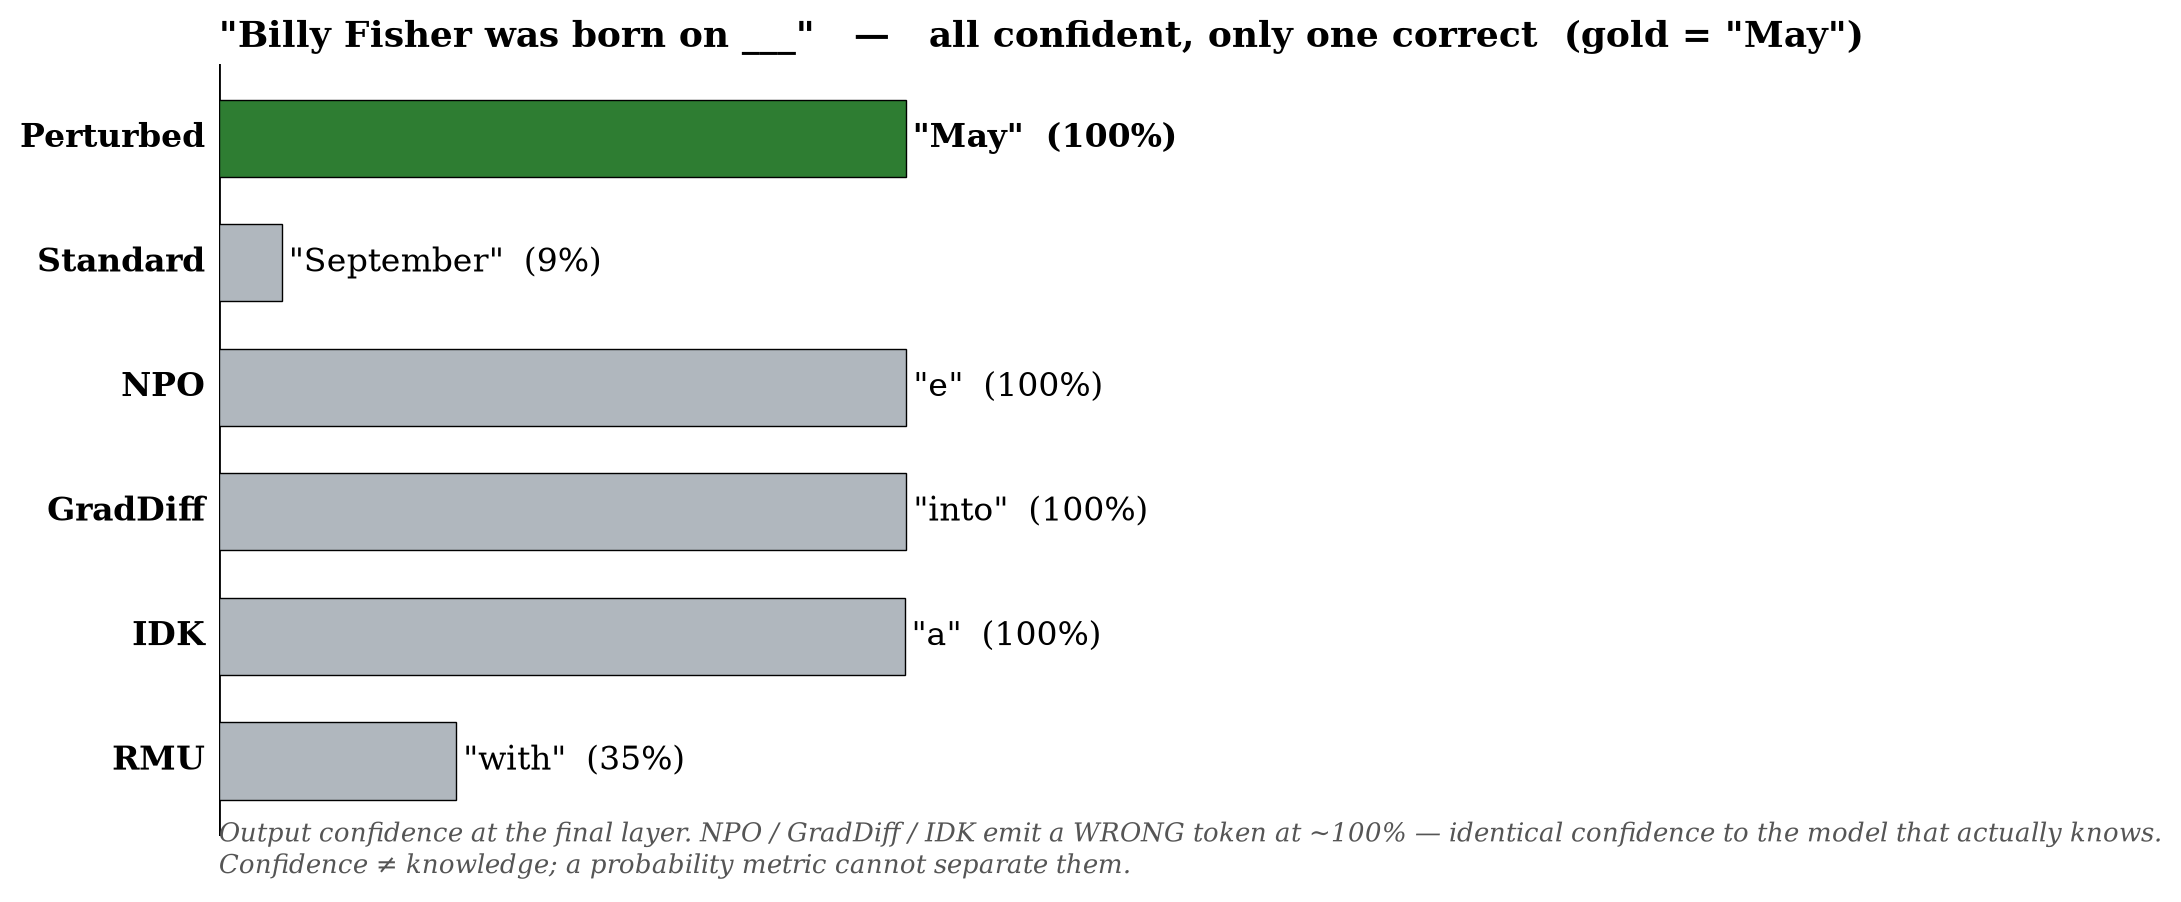
\includegraphics[width=0.85\textwidth]{lenstable_confidence_contradiction}
  \caption[Confidence is not knowledge (8B)]{Final-layer prediction across all six models. Several unlearned models are as confident in a
  wrong token as the knowing model is in the right one. Confidence does not track knowledge.}
  \label{fig:confidence}
\end{figure}

\section{A Scale-Dependent Method Verdict}
\label{sec:r-scale}

The internal readout also reveals that the same method behaves differently at different scales
(Table~\ref{tab:ranks}, 1B columns, and Figure~\ref{fig:logit1b}). At 1B only NPO drives the fact deep
(forget rank $44{,}226$); GradDiff, IDK, and RMU leave it accessible (ranks $8$ to $16$), meaning their
unlearning does not internalise at the smaller scale. This refines the output picture in an instructive
way. Infill accuracy (Table~\ref{tab:infill}) suggests IDK ``genuinely forgets'' at 1B (Unlearn $0.07$),
but the logit lens shows the fact still internally accessible there (rank~16), that is, output-suppressed
rather than erased. The overall verdict is that \emph{NPO is the most scale-robust unlearner; GradDiff and
RMU work at 8B but not at 1B; IDK is surface-level at both scales}, an ordering invisible to any output
metric and a caution against single-scale, output-only conclusions.

\begin{figure}[t]
  \centering
  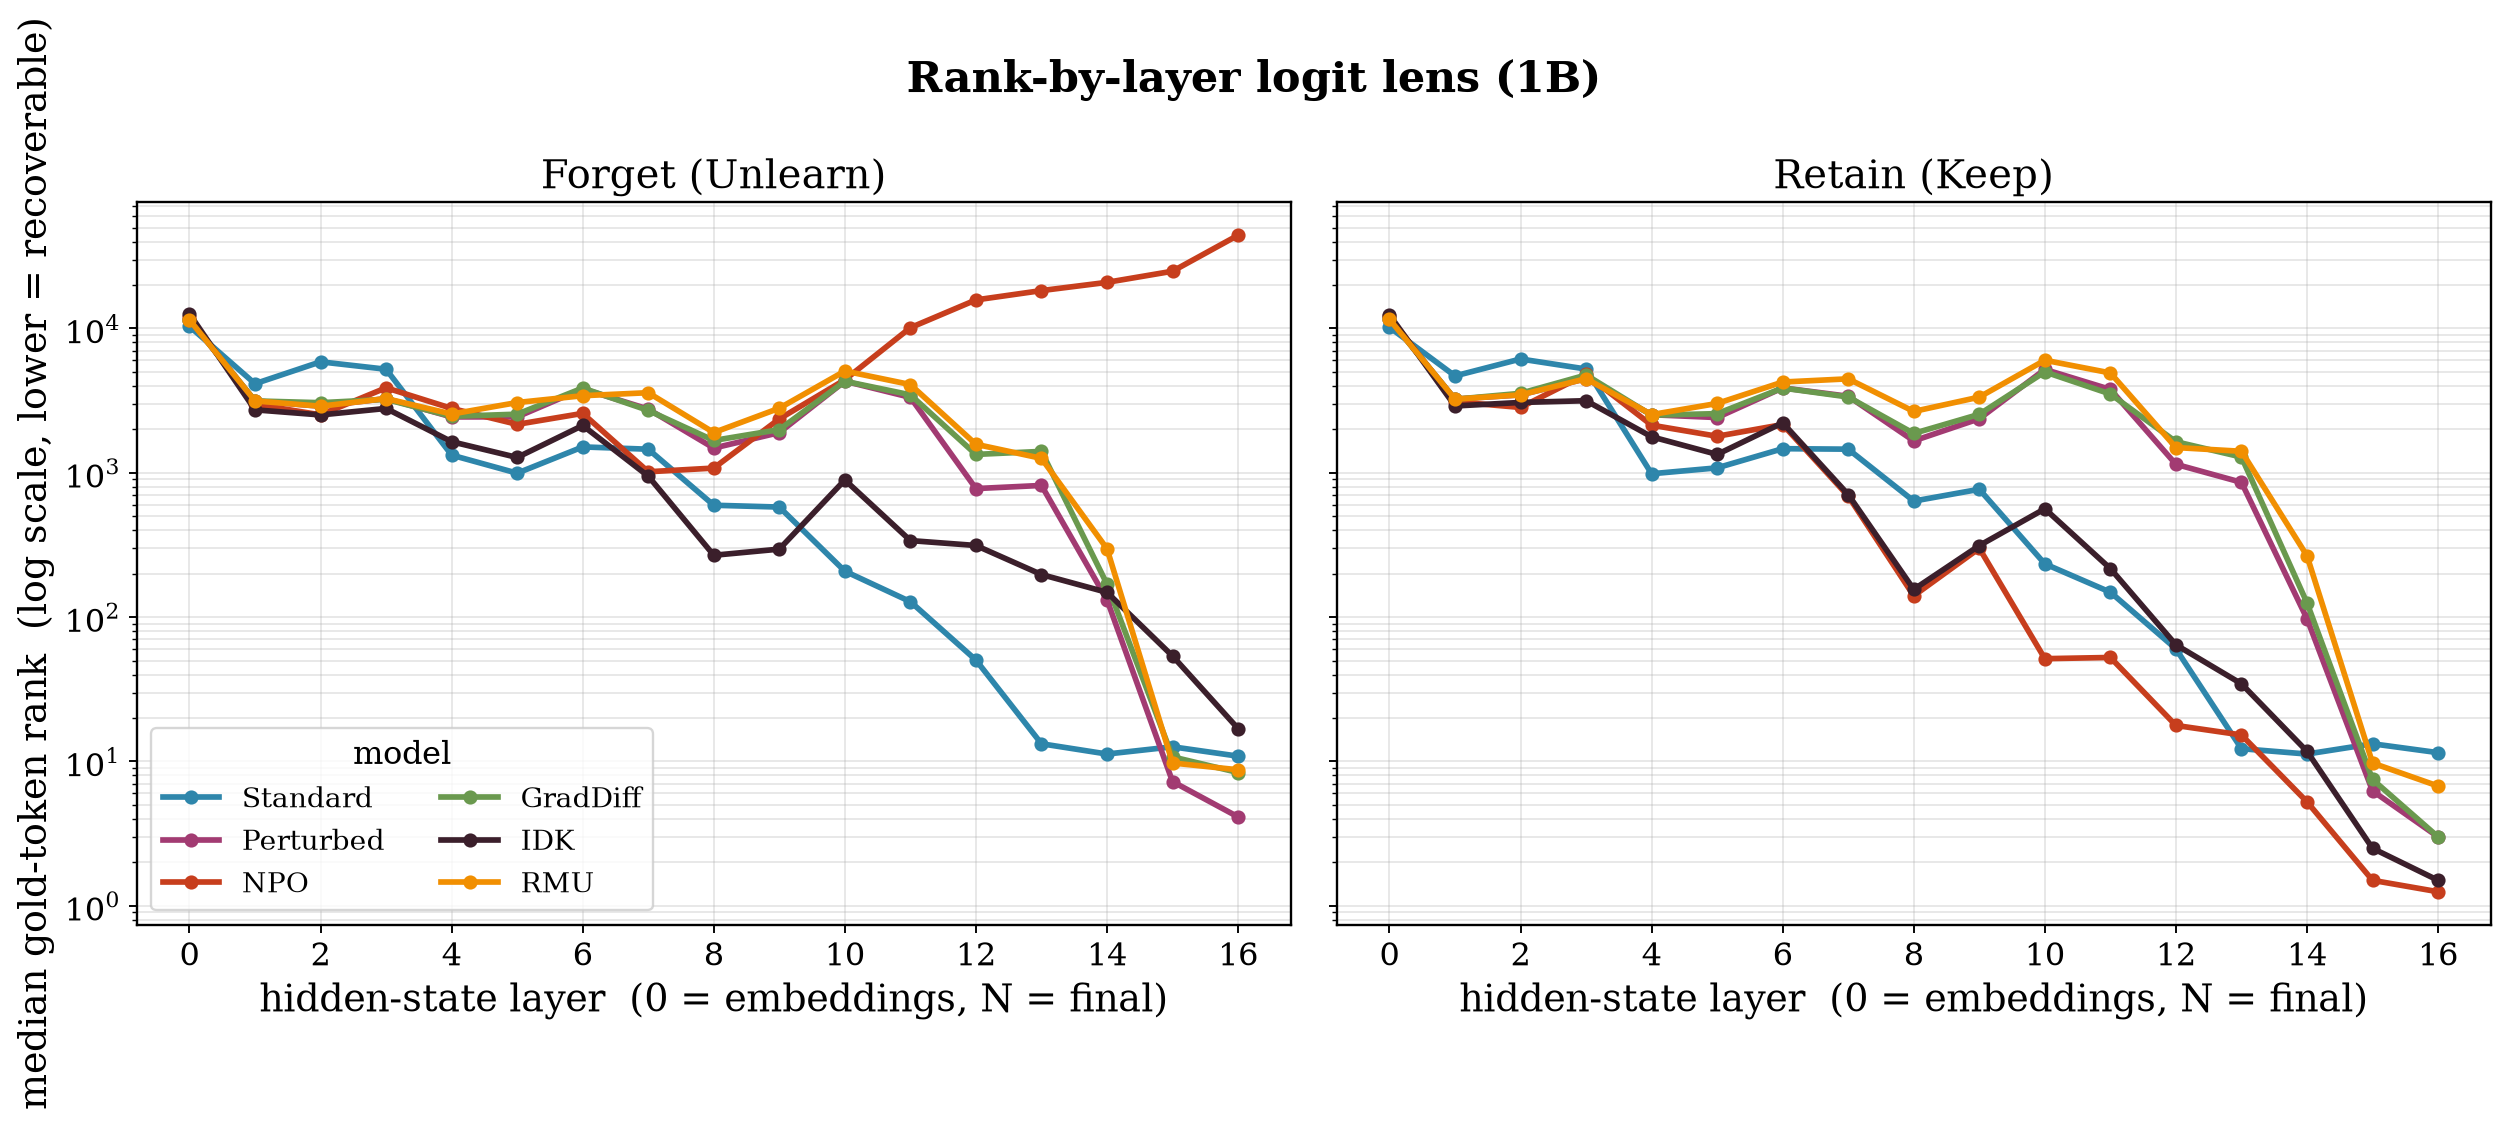
\includegraphics[width=0.92\textwidth]{logitlens_rank_median_1b}
  \caption[Rank-by-layer logit lens (1B)]{Rank-by-layer logit lens at 1B. Only NPO buries the forget fact; GradDiff, IDK, and RMU leave
  it accessible, in contrast to the 8B result of Figure~\ref{fig:logit8b}.}
  \label{fig:logit1b}
\end{figure}

\section{Mid-Stack Signatures of Four Mechanisms}
\label{sec:r-midstack}

The final-layer rank of Table~\ref{tab:ranks} is only the end of each trajectory. Reading the
\emph{mid-stack} (the minimum median rank over layers $18$ to $30$, the token's best chance of surfacing
internally) against the final rank exposes \emph{how} each method suppresses the fact
(Table~\ref{tab:midstack}). Three findings follow that the output could not show. First, the mid-stack
accessibility spans an ordering, from IDK (rank $68$) through NPO and GradDiff ($\approx 365$) to RMU
($2{,}240$). A surface-to-buried axis invisible at the output. Second, IDK barely suppresses at all. Its
token is at rank $9$ even at the output under the teacher-forced readout, so the fact remains recoverable
through to the output, and only free-generation infill hides it, the clearest case of surface-level unlearning. Third, NPO and
GradDiff share a distinctive \emph{late-suppression} signature. They keep the token accessible mid-stack
and then push it down by ten- to twenty-five-fold in the final layers, a late operation on an intact
representation, whereas RMU alone stays buried both mid-stack and at the output (ratio $1.2\times$),
consistent with its activation-scrambling at layers $5$ to $7$.

\begin{table}[t]
  \centering
  \caption[Mid-stack versus output suppression]{Mid-stack versus output suppression (8B, forget). The final/mid ratio distinguishes IDK's
  surface redirection, NPO/GradDiff's late suppression over an intact mid-stack, and RMU's deep
  suppression.}
  \label{tab:midstack}
  \begin{tabular}{lcccl}
    \toprule
    method & mid-stack min rank & final rank & final $\div$ mid & pattern \\
    \midrule
    IDK      & 68    & 9     & $0.1\times$  & no real suppression \\
    NPO      & 364   & 3{,}864 & $10.6\times$ & late / output suppression \\
    GradDiff & 370   & 9{,}192 & $24.9\times$ & late / output suppression (strongest) \\
    RMU      & 2{,}240 & 2{,}693 & $1.2\times$  & deep / early suppression \\
    \bottomrule
  \end{tabular}
\end{table}

\section{The Separation is not a Readout Artifact}
\label{sec:r-tuned}

A natural objection is that the mid-stack accessibility of Section~\ref{sec:r-midstack} is an artifact of
the logit lens's early-layer unreliability. We rule this out with the tuned lens, which re-reads the same
hidden states with a per-layer calibrated head (trained to KL/layer $\approx 0.04$).
Table~\ref{tab:tuned} shows that the tuned lens reproduces the logit-lens ordering across all six models
\emph{exactly} (Spearman correlation $1.000$), so the ordering is a property of the representations, not of
the readout. The calibrated read places every unlearned method's token at a lower absolute mid-stack rank
than the raw lens (NPO $364 \to 22$, GradDiff $370 \to 34$, RMU $2{,}240 \to 147$), while the output ranks
stay in the thousands. Because the tuned lens is trained on the output and ``skips ahead''
(Section~\ref{sec:r-lenses}), we do not read these absolute ranks as the true depth of the representation;
the load-bearing observation is the \emph{ordinal} one, that the two readouts agree on the ordering of the
models. That agreement makes the early-layer-artifact explanation unlikely. The mid-stack separation is a
property of the representations, not of any single lens. We use the tuned lens here only as an ordinal
cross-check, not as a measure of how latent the token is. Figure~\ref{fig:tunedvslogit} shows the two
readouts side by side.

\begin{table}[t]
  \centering
  \caption[Tuned versus logit lens, mid-stack rank]{Tuned lens versus logit lens (8B, forget), mid-stack minimum rank. The ordering is identical
  (Spearman $1.000$); we read only this ordering agreement, not the calibrated lens's absolute ranks.}
  \label{tab:tuned}
  \begin{tabular}{lccc}
    \toprule
    model & logit mid-min & tuned mid-min & final (both) \\
    \midrule
    Perturbed \emph{(knows)}     & 1 & 1 & 1 \\
    IDK                          & 9 & 9 & 9 \\
    Standard \emph{(never knew)} & 10 & 10 & 10 \\
    NPO      & 364   & \textbf{22}  & 3{,}864 \\
    GradDiff & 370   & \textbf{34}  & 9{,}192 \\
    RMU      & 2{,}240 & \textbf{147} & 2{,}693 \\
    \bottomrule
  \end{tabular}
\end{table}

\begin{figure}[t]
  \centering
  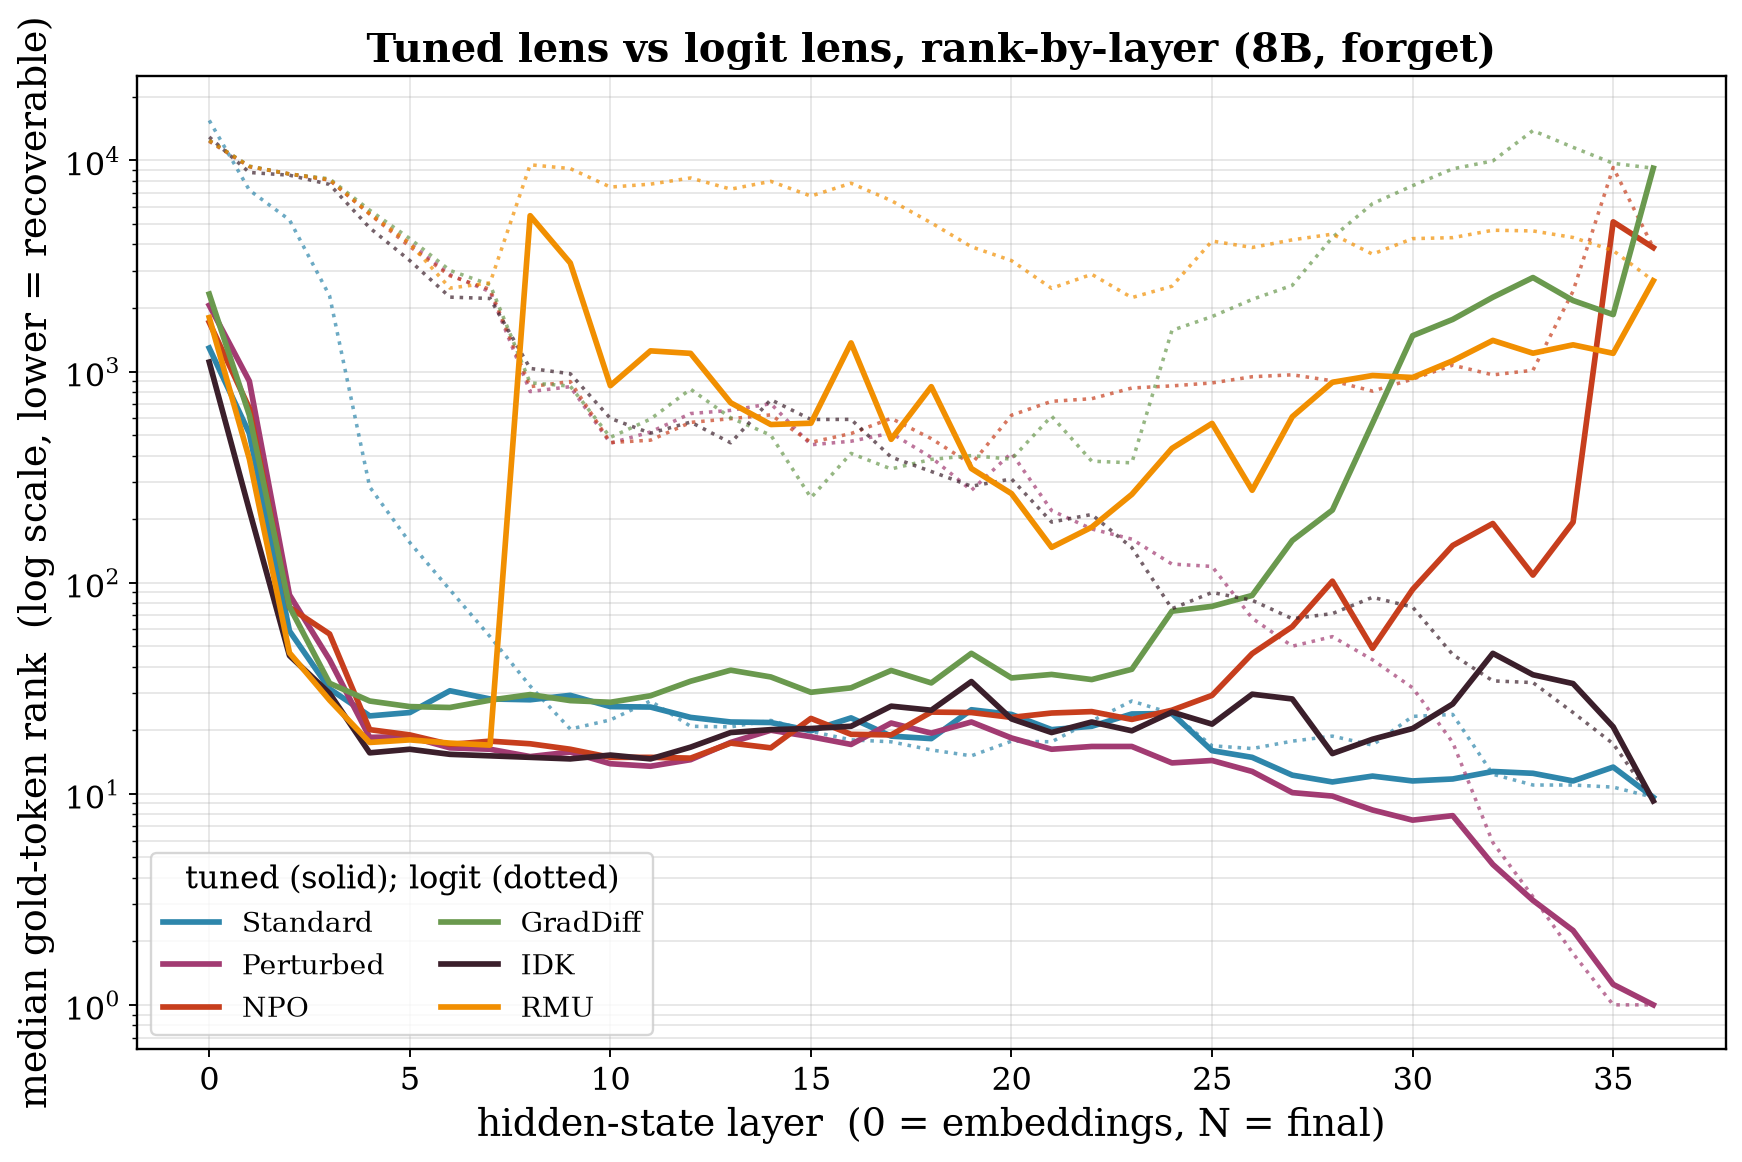
\includegraphics[width=0.72\textwidth]{tuned_vs_logit_8b}
  \caption[Tuned versus logit lens, rank-by-layer (8B)]{Tuned lens (solid) versus logit lens (dotted), rank-by-layer at 8B. The calibrated lens
  preserves the ordering, confirming that the mid-stack accessibility is a property of the representations,
  not of the readout.}
  \label{fig:tunedvslogit}
\end{figure}

\section{\texorpdfstring{$D_\text{mech}$}{D\_mech} is the Most Faithful Metric on Hubble-8B}
\label{sec:r-faithful}

We now put $D_\text{mech}$ through the faithfulness meta-evaluation of Section~\ref{sec:m-metaeval},
against the na\"ive internal metric and nine established output and lexical metrics.
Table~\ref{tab:faithful} reports the two effect sizes and their combination. Discrimination is easy, and
almost every metric separates the knows pool from the absent pool ($\text{discrim} > 0.8$ for most).
Invariance is where they part. Under a meaning-preserving rewording, the lexical metrics collapse, 
gold-answer probability falls from $0.948$ to $0.164$, and ROUGE and extraction strength fall to zero,
so the still-knowledge-present Paraphrased cell comes to look like the negatives, whereas $D_\text{mech}$
shifts far less, from $1.213$ to $0.921$. Its invariance shift is $0.466$, a large reduction but not zero,
against $\geq 0.95$ for all ten other metrics; on Hubble-8B it is the only metric that is at once strongly
discriminative and paraphrase-stable. Its composite faithfulness score, $0.442$, is about eighteen times the
best lexical metric (truth ratio, $0.025$). The composite has a small denominator, so this multiplier is a
summary statistic rather than an absolute unit; the primary evidence is the two effect sizes, reported
separately. On Hubble-8B this ranking does not depend on the multiplicative form: $D_\text{mech}$ stays
first under additive, harmonic-mean, minimum, and invariance-as-constraint aggregations
(Section~\ref{sec:r-crossbench}). Bootstrapping over facts ($4000$ resamples, holding the fitted anchors
fixed, so these are fact-resampling intervals conditional on the anchors rather than a full anchor-uncertainty
bootstrap) puts $D_\text{mech}$'s faithfulness at $0.442$ with a $95\%$ CI of $[0.311, 0.558]$, which does
not overlap the best lexical metric's $[0.000, 0.072]$, so the advantage is not an artifact of the point
estimate. Figures~\ref{fig:fig4} and~\ref{fig:scatterbar} show the full distributions and the
invariance-discrimination trade-off.

\begin{table}[t]
  \centering
  \caption[Faithfulness meta-evaluation (Hubble-8B)]{Faithfulness meta-evaluation (8B, $n=44$). A faithful metric needs low invariance shift and
  high discrimination. Only $D_\text{mech}$ has both.}
  \label{tab:faithful}
  \begin{tabular}{llccc}
    \toprule
    metric & family & invar.\ shift $\downarrow$ & discrim.\ $\uparrow$ & faithful $\uparrow$ \\
    \midrule
    \textbf{$D_\text{mech}$} & \textbf{mechanistic} & \textbf{0.466} & 0.827 & \textbf{0.442} \\
    truth\_ratio         & lexical & 0.974 & 0.973 & 0.025 \\
    rouge                & lexical & 0.975 & 0.494 & 0.012 \\
    extraction\_strength & lexical & 0.976 & 0.505 & 0.012 \\
    exact\_mem           & lexical & 0.991 & 0.818 & 0.008 \\
    probability          & lexical & 0.999 & 0.928 & 0.001 \\
    min\_rank            & mechanistic & 1.000 & 0.892 & 0.000 \\
    mia (loss/mink/minkpp/zlib) & lexical & 0.95 to 0.99 & 0.16 to 0.31 & $\leq$0.008 \\
    \bottomrule
  \end{tabular}
\end{table}

Two points deserve emphasis. First, the win is the \emph{distance construction}, not merely ``use
internals'': the na\"ive internal metric $\min$-rank \emph{fails} invariance (shift $1.000$), because
rewording shifts the absolute rank consistently, whereas $D_\text{mech}$ is far more paraphrase-stable
because it is relative and the anchor subtraction cancels most of the common-mode shift. Second, this is the
empirical
confirmation, on the benchmark's own terms and against ten established metrics, of the thesis's central
claim that output and lexical metrics conflate surface form with knowledge.

\begin{figure}[t]
  \centering
  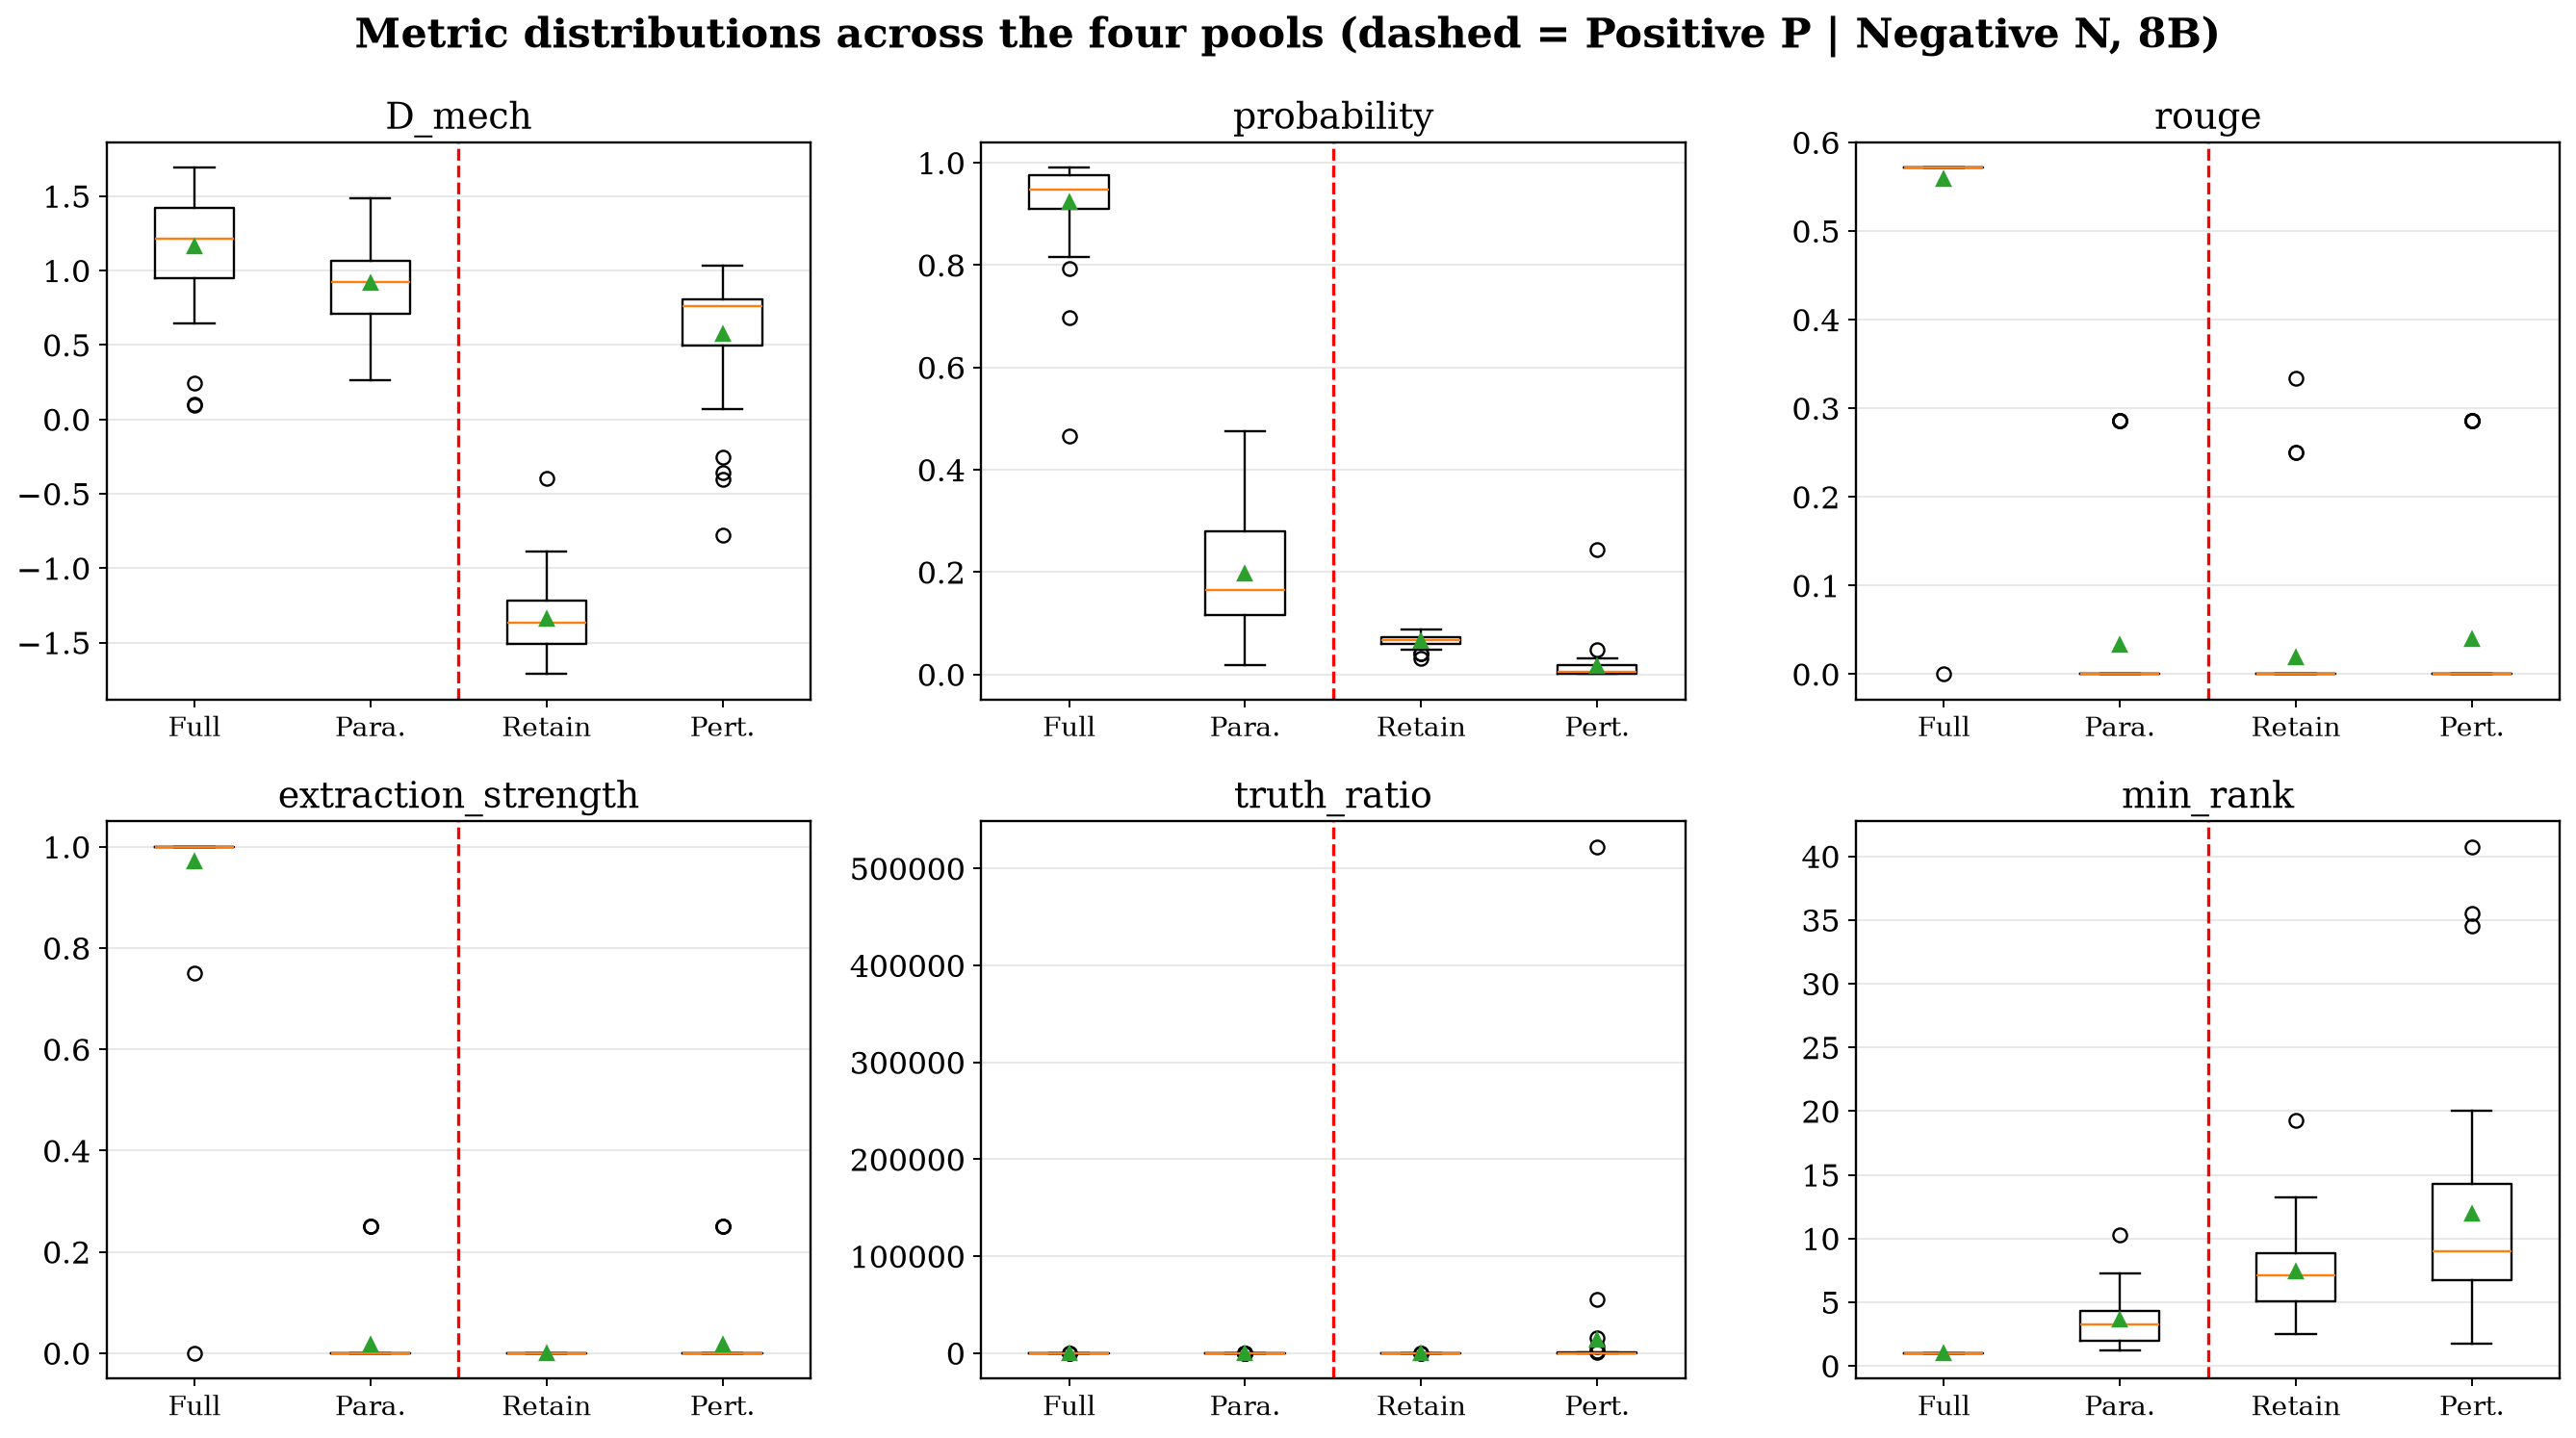
\includegraphics[width=0.95\textwidth]{mech_metaeval_fig4}
  \caption[Metric distributions across the four pools]{Distribution of each metric across the four pools (dashed line separates Positive from
  Negative). A faithful metric keeps Full $\approx$ Paraphrased and shows a Positive-Negative gap;
  $D_\text{mech}$ does both, while the lexical metrics let the Paraphrased cell collapse toward the
  negatives.}
  \label{fig:fig4}
\end{figure}

\begin{figure}[t]
  \centering
  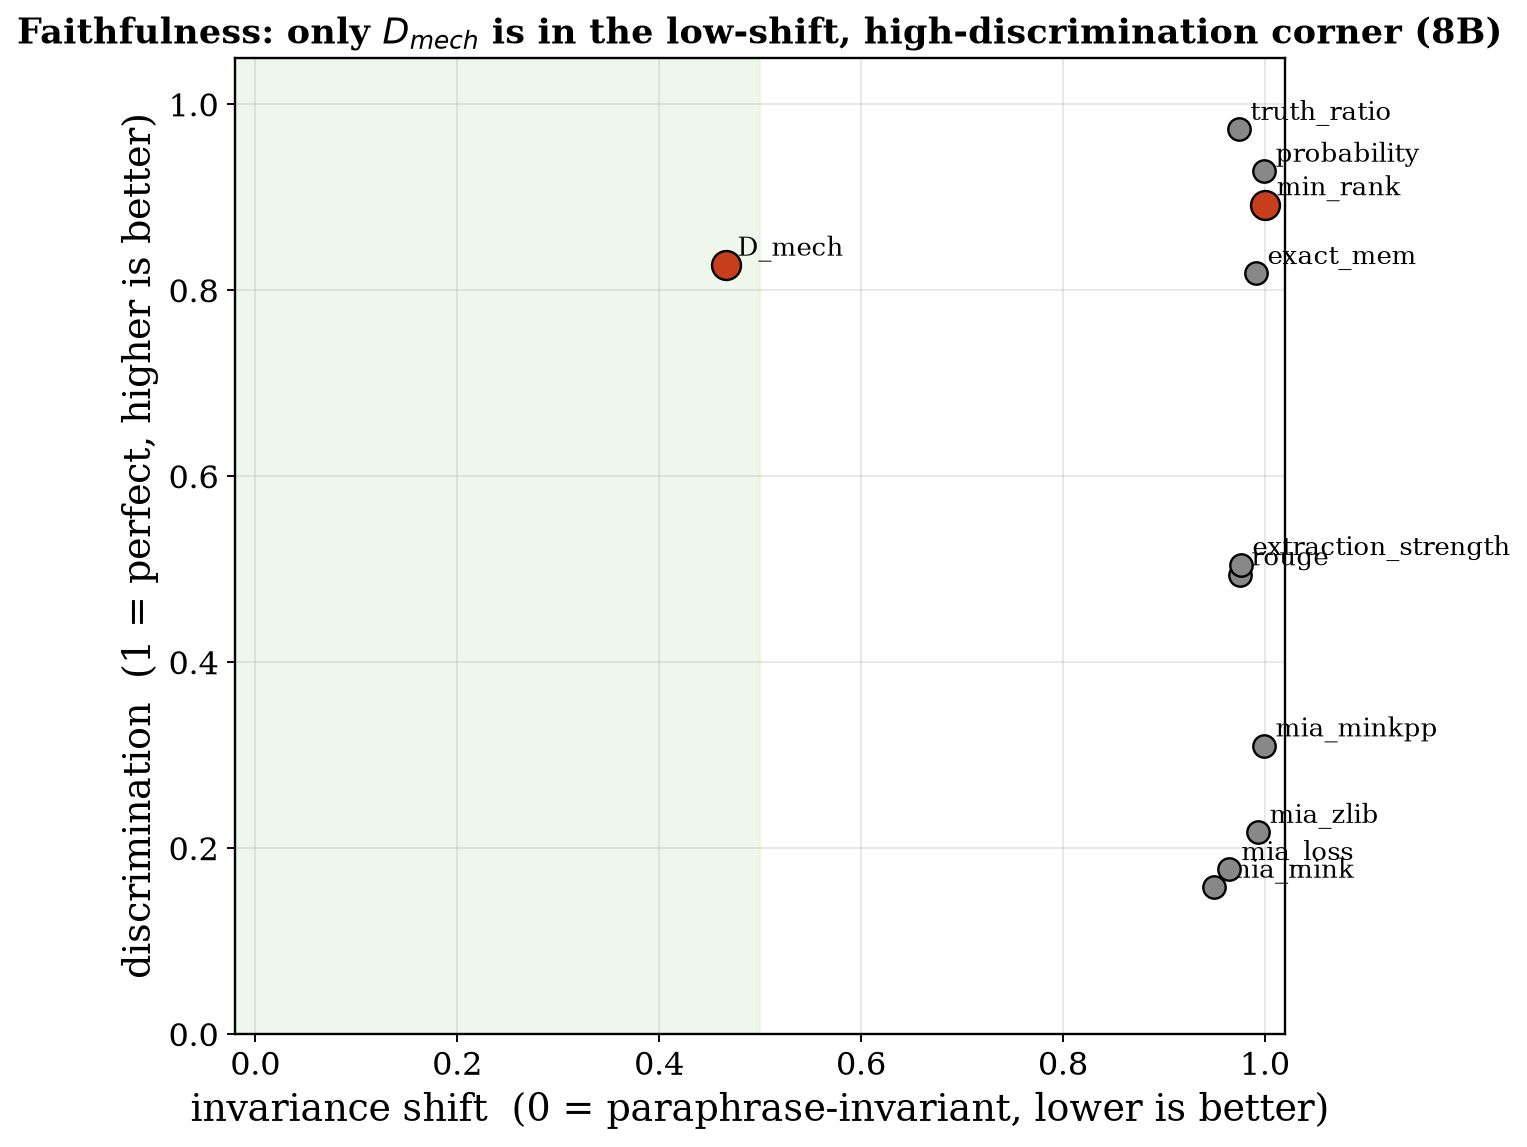
\includegraphics[width=0.48\textwidth]{mech_invar_discrim_scatter}\hfill
  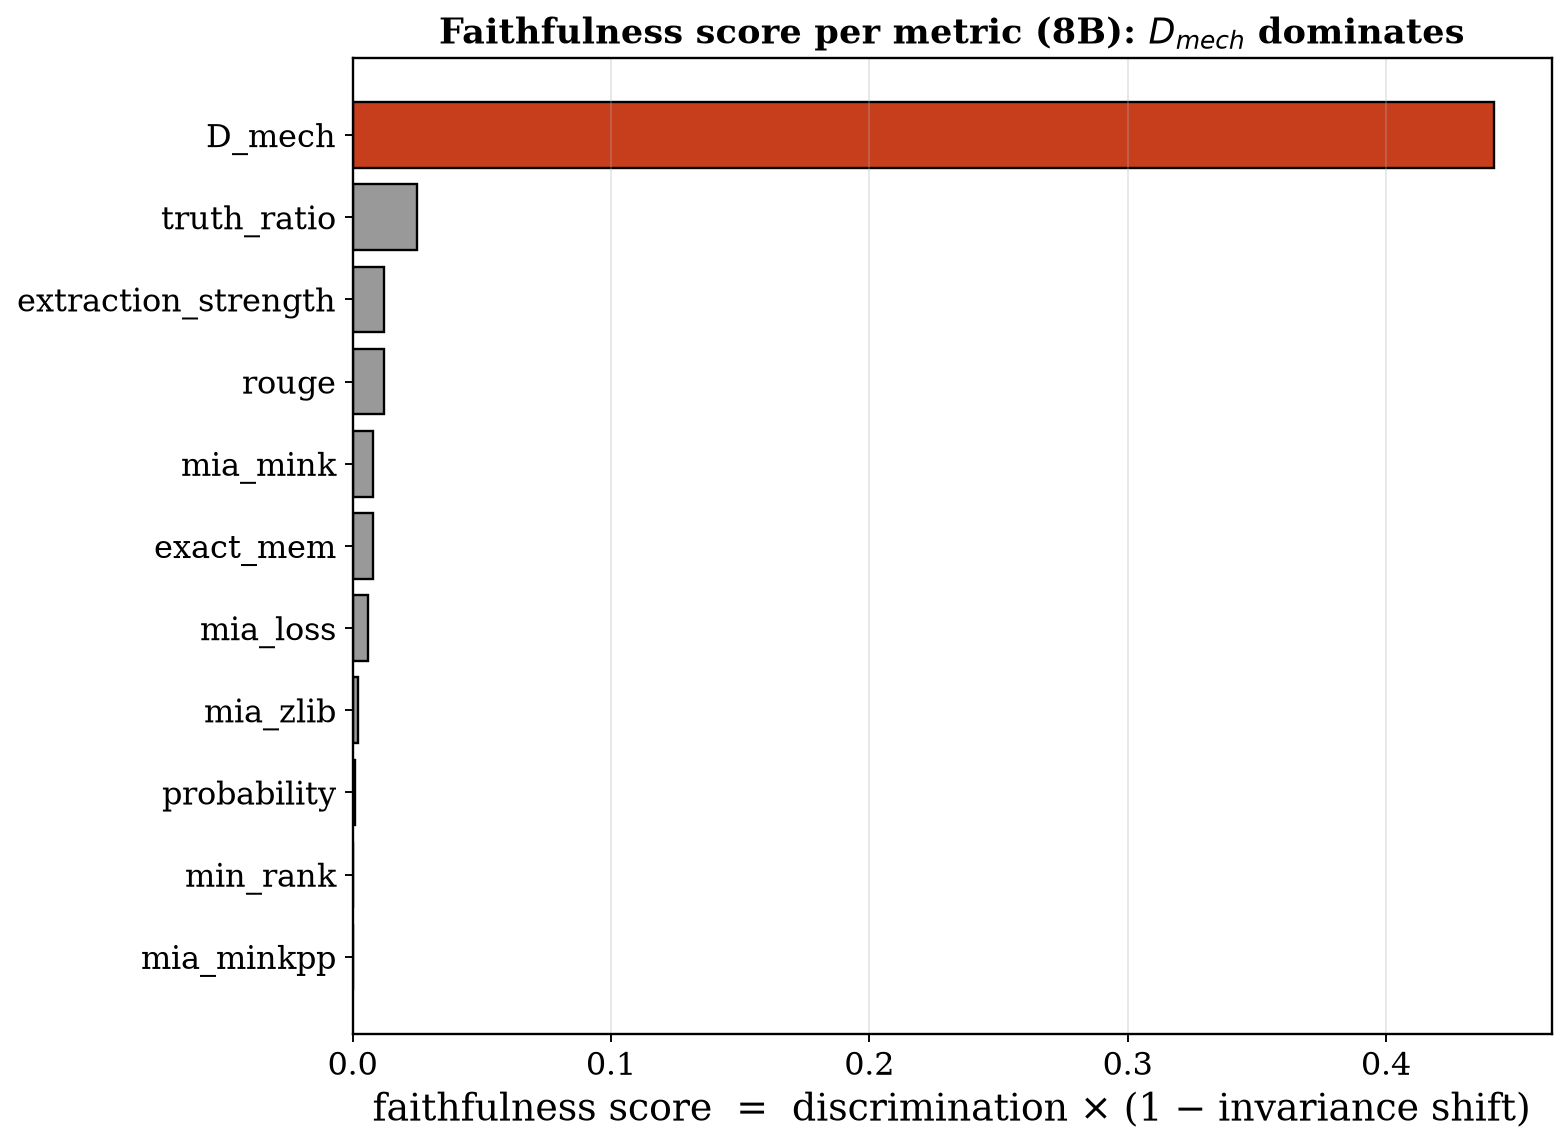
\includegraphics[width=0.48\textwidth]{mech_faithful_bar}
  \caption[Invariance, discrimination, and faithfulness]{Left. Invariance shift versus discrimination; only $D_\text{mech}$ sits in the faithful corner
  (low shift, high discrimination). Right. Faithfulness score per metric; $D_\text{mech}$ is about
  far above the best lexical metric.}
  \label{fig:scatterbar}
\end{figure}

\section{Paraphrase Stability}
\label{sec:r-invariance}

Figure~\ref{fig:worked} isolates the deciding criterion on a single fact. With the knowledge unchanged and
only the wording reworded, the gold-answer probability collapses from $0.95$ to $0.16$ (a near-total shift)
while $D_\text{mech}$ changes far less, staying positive ($1.21 \to 0.92$). Figure~\ref{fig:showcase}
generalises this to
four rewordings of the same fact. The surface readouts (gold probability, ROUGE) swing widely across the
phrasings, yet the gold month emerges the same way inside the model and $D_\text{mech}$ stays positive
throughout. A multi-paraphrase robustness check confirms the pattern quantitatively. Averaged over several
meaning-preserving rewordings, $D_\text{mech}$'s invariance shift stays the lowest while the lexical metrics
swing. The paired change tells the same story. Across the $44$ facts, the Full-to-Paraphrased change in
$D_\text{mech}$ has median $-0.24$, and $D_\text{mech}$ stays positive, that is on the knows side of the
zero boundary, for every fact; the shift is statistically detectable (paired Wilcoxon $p<0.001$) but small
next to the anchor gap, which is exactly the reduced sensitivity the metric is designed to have.

\begin{figure}[t]
  \centering
  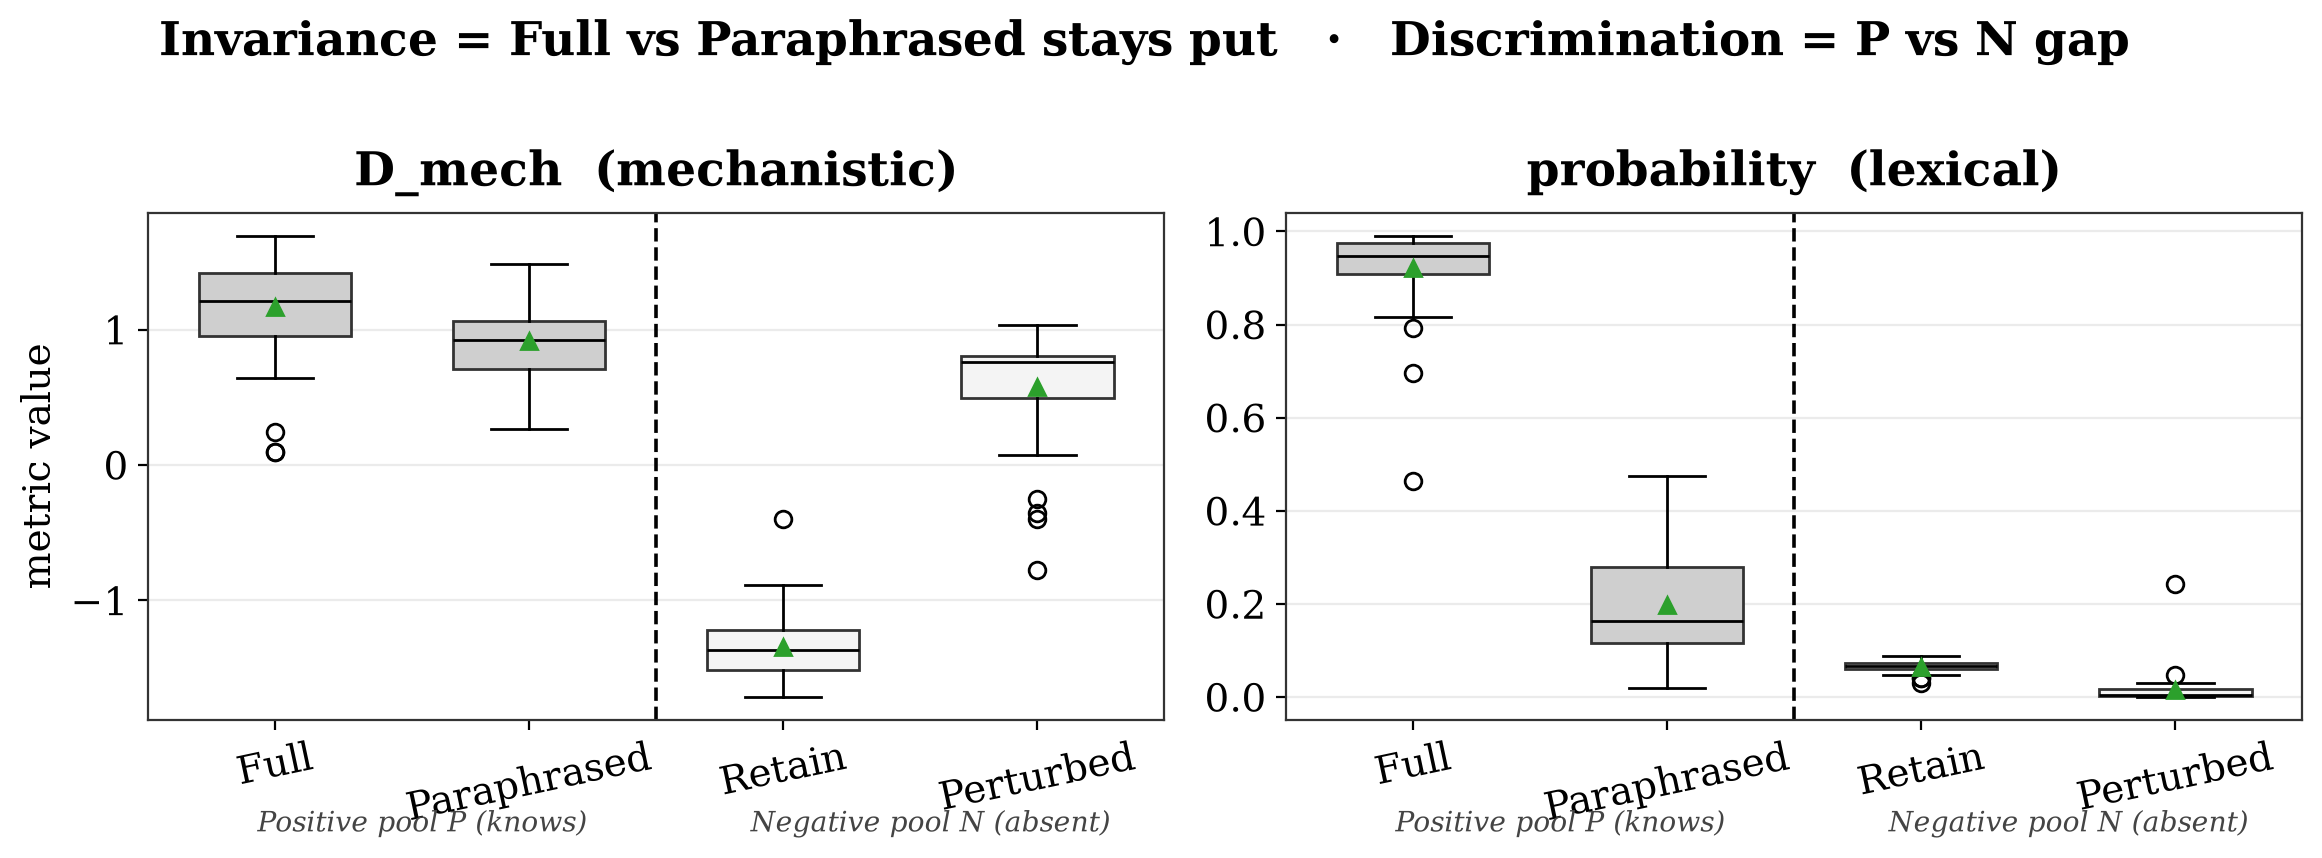
\includegraphics[width=0.9\textwidth]{mech_worked_example}
  \caption[Worked paraphrase-stability example (8B)]{Same knowledge, reworded prompt. The gold-answer
  probability shifts almost completely ($0.95 \to 0.16$), whereas $D_\text{mech}$ remains positive and
  changes substantially less ($1.21 \to 0.92$). Both separate knows from absent, so paraphrase stability is
  the deciding test.}
  \label{fig:worked}
\end{figure}

\begin{figure}[t]
  \centering
  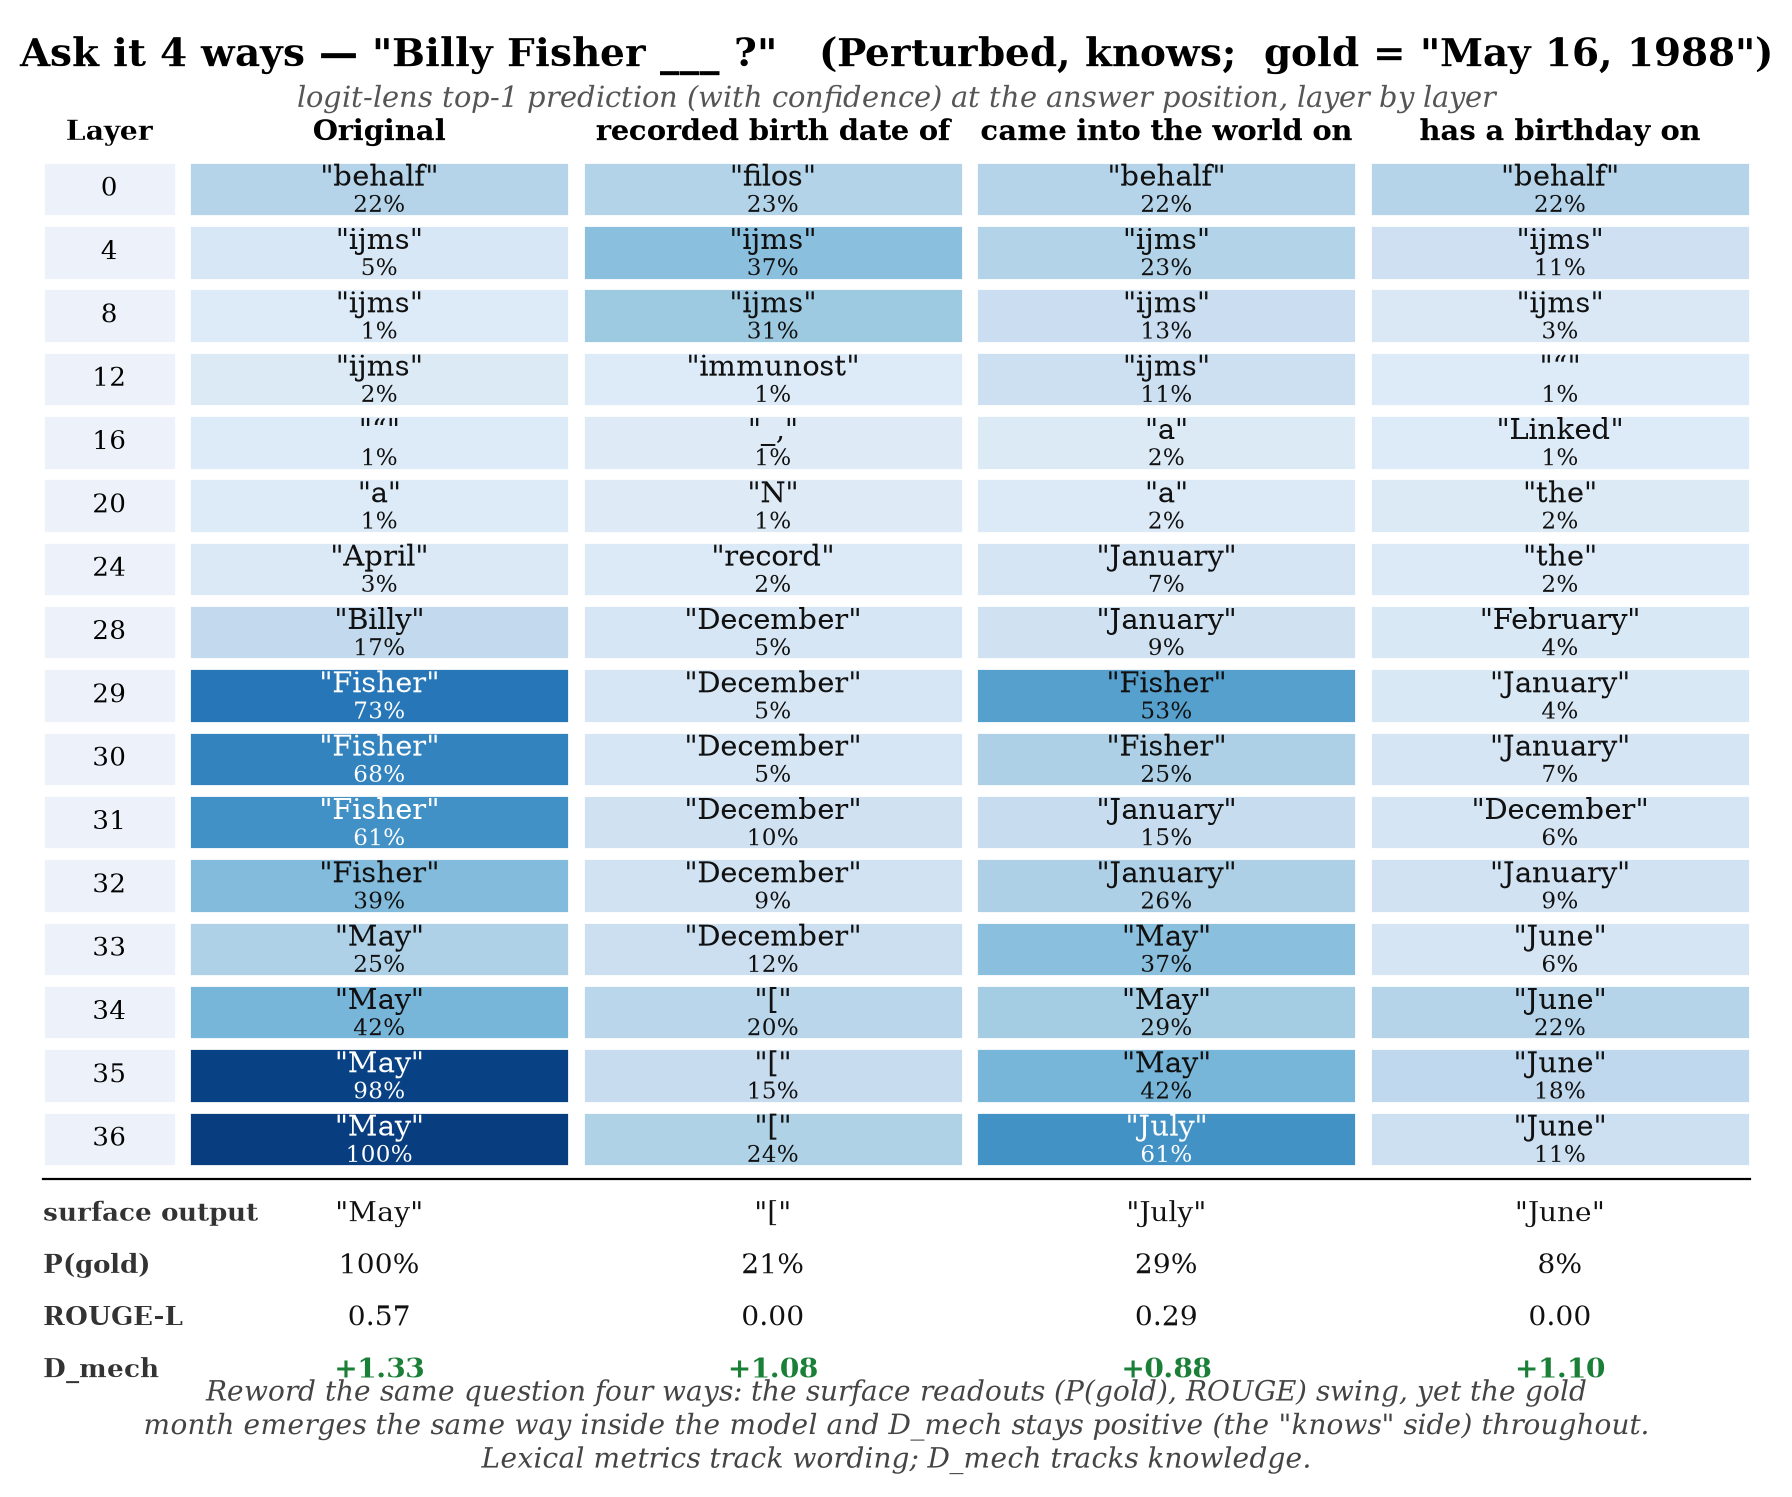
\includegraphics[width=0.85\textwidth]{paraphrase_showcase_ent0_8b}
  \caption[One fact asked four ways (8B)]{One fact asked four ways (Perturbed, 8B). Surface readouts swing across phrasings while the gold
  month emerges the same way internally and $D_\text{mech}$ stays positive. Lexical metrics track wording,
  $D_\text{mech}$ tracks knowledge.}
  \label{fig:showcase}
\end{figure}

\section{Comparing the Three Lenses}
\label{sec:r-lenses}

Finally, Figure~\ref{fig:lenscompare} compares the logit, tuned, and Jacobian lenses on the same $44$
facts. The tuned lens sits at a low rank ($\approx 10$) from the very first layer for \emph{every} model,
including the suppressed NPO and GradDiff. Because it is trained on the output, it ``skips ahead'',
laundering the answer into every layer and hiding both where the computation happens and the suppression
itself. It is therefore a poor basis for a knowledge probe, which is exactly why $D_\text{mech}$ is built
on the logit lens rather than the calibrated tuned lens. We use the tuned lens only as an ordinal
cross-check between models, not as a readout of where or when the answer is computed. The logit lens shows
genuine emergence, and the Jacobian lens, a first-order readout grounded in the model's local
input-output sensitivity rather than a trained decoder (Figure~\ref{fig:jacobian}), is smooth and
well-ordered, reproducing the taxonomy (the knowing model reaches rank~1, the never-knew model plateaus
higher, and the suppressors rise again in the final layers, the signature of active output suppression).
For NPO in particular the Jacobian lens keeps the fact buried at every layer even though the logit lens
still detects a lingering linear trace, illustrating the difference between a correlational readout and a
sensitivity-based one. Because the Jacobian lens is an averaged first-order approximation around reference
states, we treat it as interventionally grounded and confirmatory, not as proof that the representation is
causally necessary for the output.

\begin{figure}[t]
  \centering
  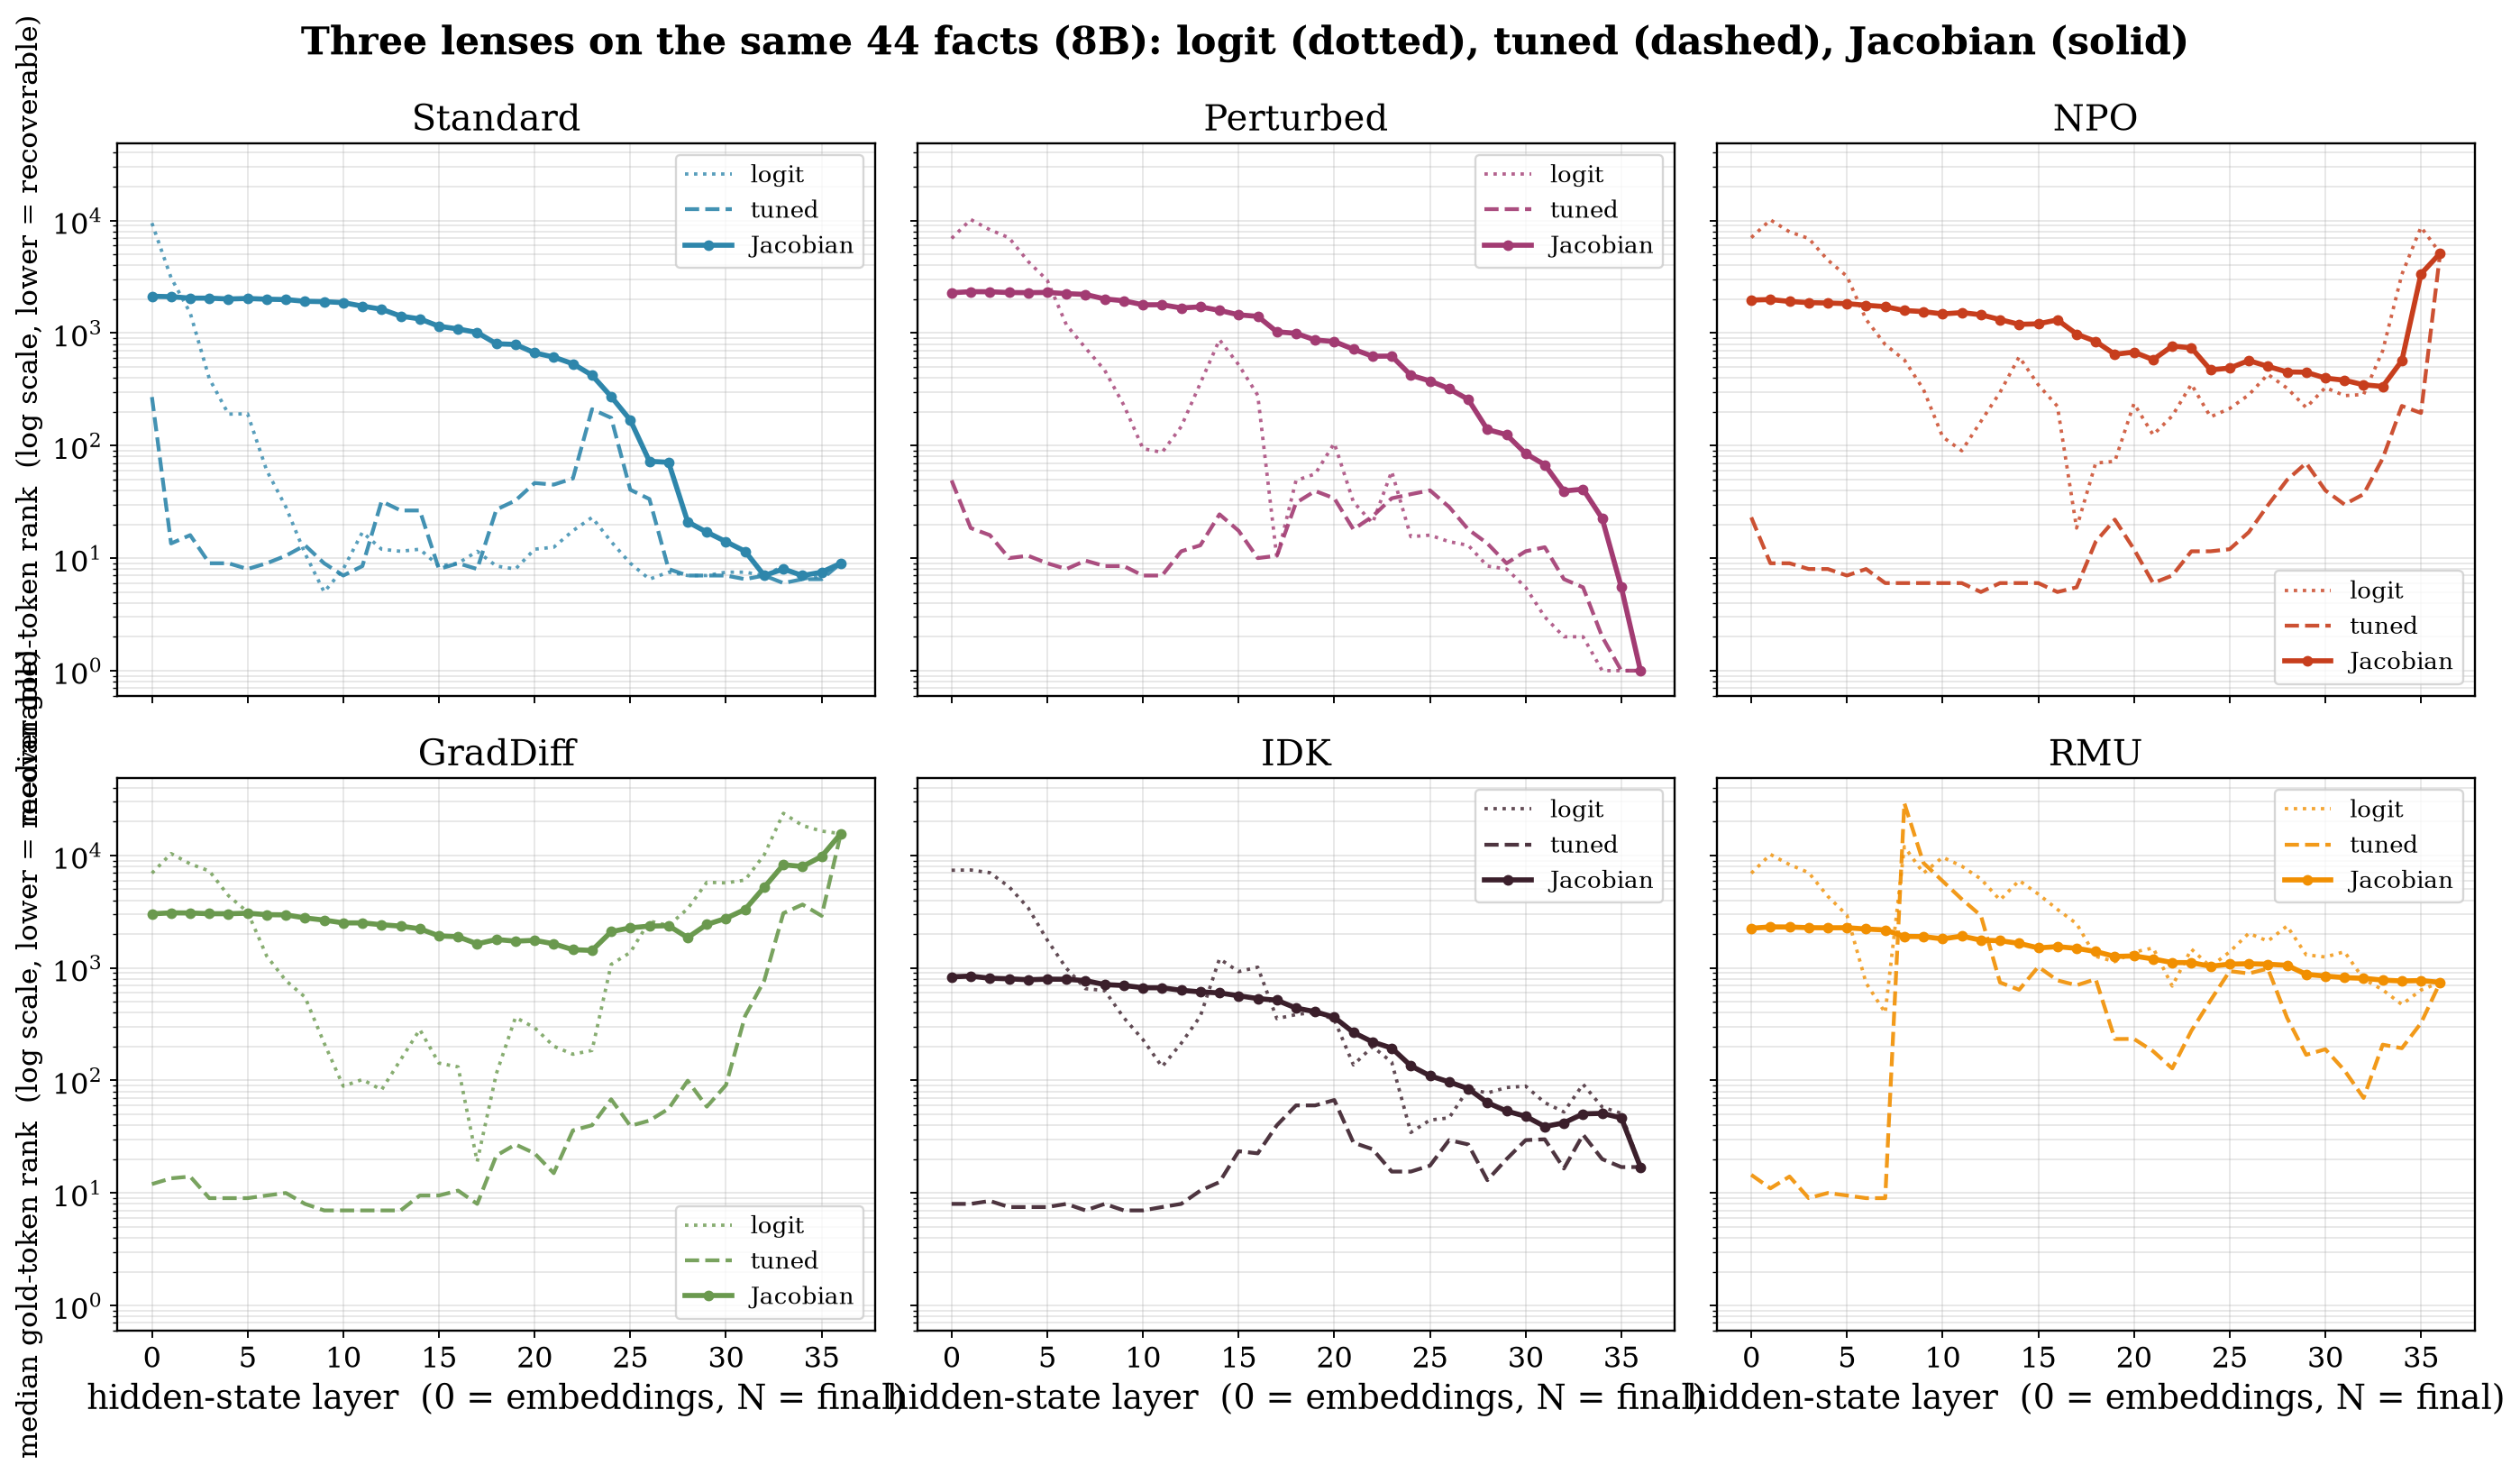
\includegraphics[width=0.98\textwidth]{lens_compare_8b}
  \caption[The three lenses compared (8B)]{The three lenses on the same $44$ facts (8B). The tuned lens (dashed) sits near rank $10$ from
  layer $0$ for every model, even the suppressed ones (it ``skips ahead''); the logit lens (dotted) shows
  emergence; the Jacobian lens (solid) is smooth and sensitivity-based.}
  \label{fig:lenscompare}
\end{figure}

\begin{figure}[t]
  \centering
  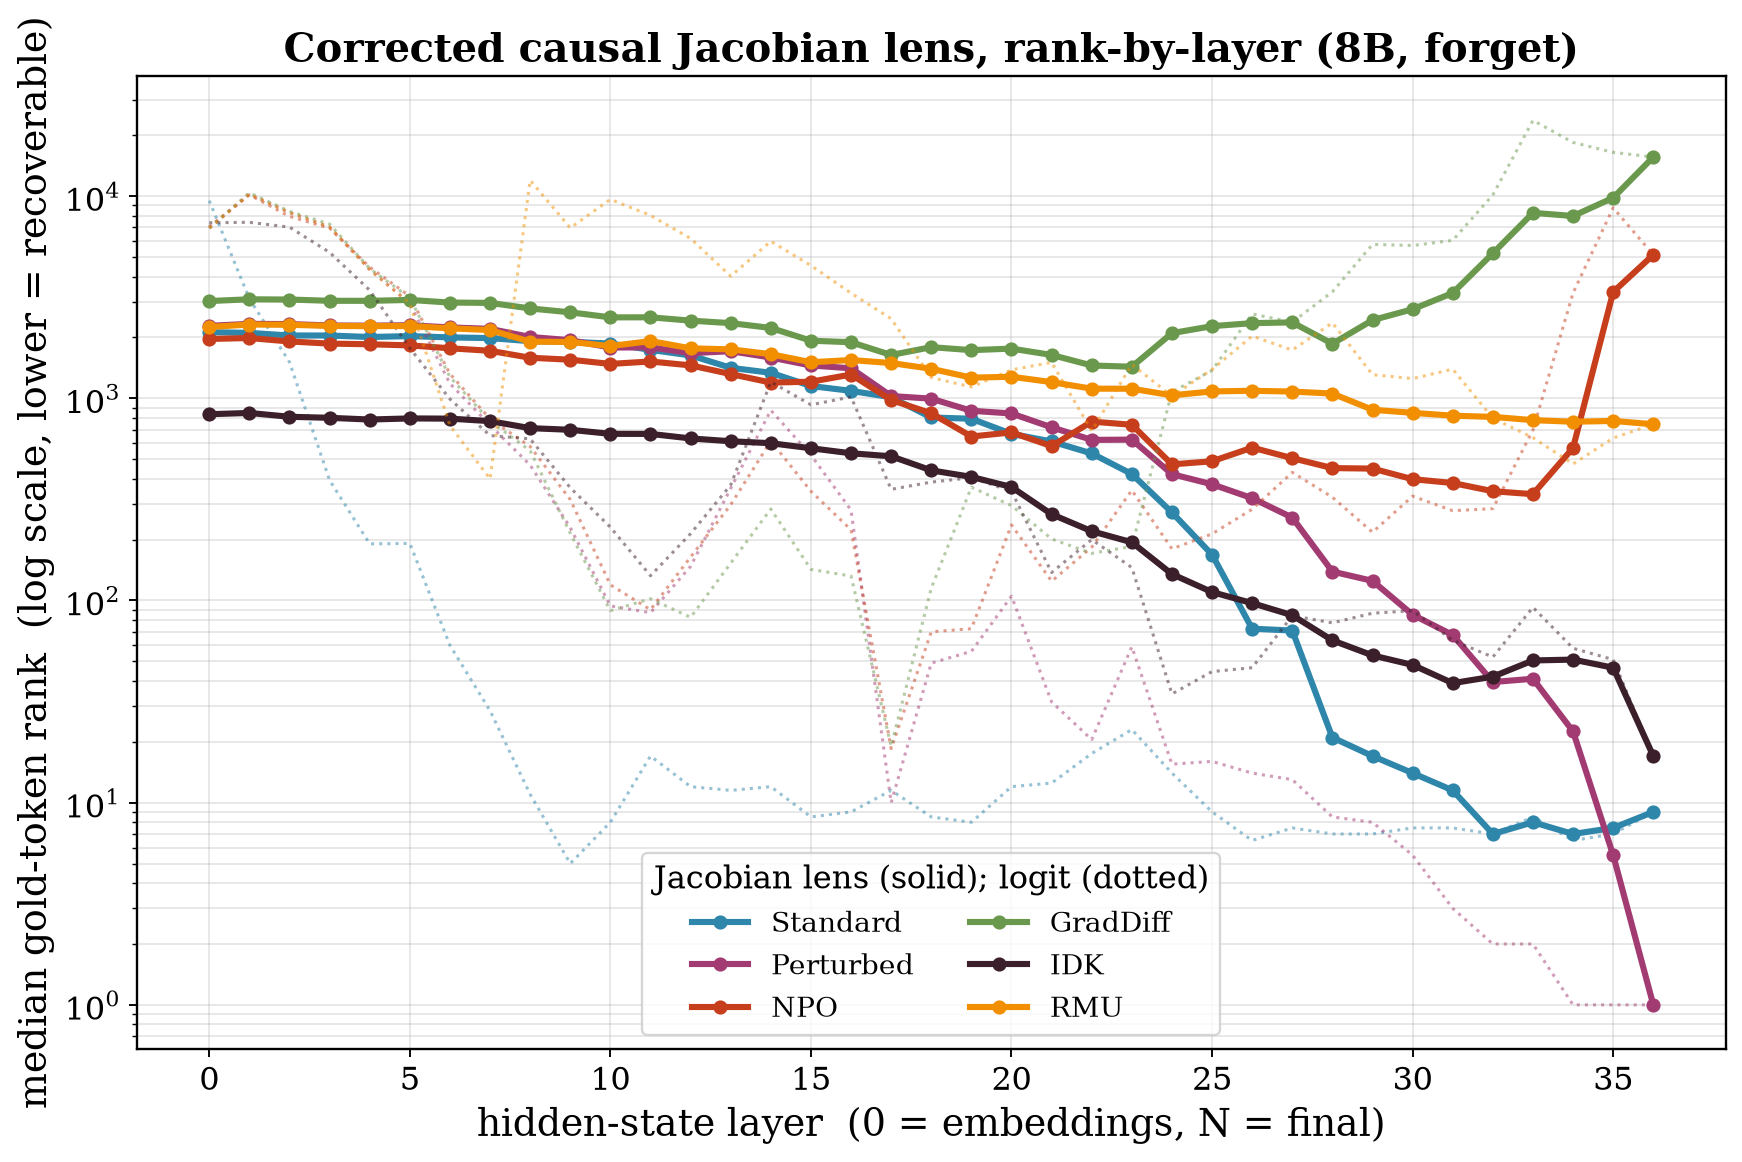
\includegraphics[width=0.8\textwidth]{jlens_affine_rank_8b}
  \caption[Corrected Jacobian lens (8B)]{The corrected Jacobian lens (a first-order, interventionally-grounded readout) at 8B reproduces
  the taxonomy with a smooth, ordered readout, including the late-layer rise for the suppressor methods that
  marks active output suppression.}
  \label{fig:jacobian}
\end{figure}

\section{Robustness of the Faithfulness Result and a Second Benchmark}
\label{sec:r-crossbench}

Two properties decide how much weight the Hubble-8B result of Section~\ref{sec:r-faithful} can carry. The
first is whether the ranking depends on the composite formula, and the second is whether it survives a
change of benchmark and model family. We test both.

\paragraph{The Hubble-8B conclusion is robust to the aggregation formula.}
The faithful score $\text{discrim}\cdot(1-\text{invar\_shift})$ is one of several reasonable ways to combine
the two effect sizes. We recompute the ranking under four alternatives, an additive score
$\text{discrim}+(1-\text{invar\_shift})$, the harmonic mean of the two components, their minimum, and an
invariance-as-constraint rule that ranks by discrimination among metrics with $\text{invar\_shift}<0.5$. On
Hubble-8B, $D_\text{mech}$ is first under all five (Table~\ref{tab:agg}); at every scale and benchmark it is
the best mechanistic metric and beats every standard output metric under every formula (the sole exception
is the additive score at Hubble-1B). The eighteen-fold gap is thus a property of the data, not of the
multiplication.

\begin{table}[t]
  \centering
  \caption[$D_\text{mech}$ rank under five aggregations]{Rank of $D_\text{mech}$ (of $11$ metrics) under five aggregations of the two effect sizes.
  Except for the additive score at Hubble-1B, $D_\text{mech}$ is the best mechanistic metric and beats
  every standard output metric in every cell.}
  \label{tab:agg}
  \begin{tabular}{lccccc}
    \toprule
    benchmark & product & additive & harmonic & minimum & constraint \\
    \midrule
    Hubble-8B & \textbf{1} & \textbf{1} & \textbf{1} & \textbf{1} & \textbf{1} \\
    Hubble-1B & 2 & 4 & 2 & 2 & 2 \\
    TOFU-1B   & 4 & 4 & 4 & 4 & 2 \\
    TOFU-3B   & 5 & 5 & 5 & 5 & 3 \\
    TOFU-8B   & 4 & 4 & 4 & 4 & 2 \\
    \bottomrule
  \end{tabular}
\end{table}

\paragraph{A second benchmark and model family.}
We repeat the full meta-evaluation on the OpenUnlearning TOFU benchmark, whose forget set is
fictitious-author question-answer pairs with multi-token sentence answers, using the released \texttt{full}
(knows) and \texttt{retain90} (never-knew) checkpoints as anchors at 1B, 3B, and 8B. The four pools are the
TOFU analogues of Section~\ref{sec:m-metaeval}, namely the knows model on the canonical and on a reworded question,
the never-knew model, and the knows model scored against a wrong answer. $D_\text{mech}$ is faithful at all
three scales (Table~\ref{tab:tofu}). It discriminates strongly ($p<10^{-45}$), its invariance shift
($0.35$ to $0.42$) is far below that of the generation-overlap and answer-probability metrics ($0.80$ to
$0.97$), and at every scale it is the best internal metric and above every generation-overlap and
answer-probability metric (ROUGE, exact-match, extraction strength, and gold-answer probability). It is not,
on TOFU, the single best metric overall. A few likelihood-based aggregates, the truth ratio and the loss-
and zlib-based membership-inference scores, are also paraphrase-stable here and score slightly higher on the
composite. The two are in fact statistically comparable on TOFU-8B: $D_\text{mech}$'s fact-resampling
faithfulness CI $[0.456, 0.645]$ overlaps the truth ratio's $[0.578, 0.729]$, while both sit far above the
direct answer-probability metric (probability $[0.002, 0.073]$). This difference from Hubble is expected.
TOFU rewords the entire question and scores a multi-token answer, so metrics that aggregate over the whole
answer are less exposed to a single-token surface shift than they were under Hubble's trigger-only rewording.
The claim that travels is therefore the calibrated one. Across the two benchmarks evaluated, $D_\text{mech}$
separates knowledge from surface form better than the direct generation and answer-probability metrics,
while its margin over the strongest likelihood-based aggregates is benchmark-dependent.

\begin{table}[t]
  \centering
  \caption[TOFU meta-evaluation (1B/3B/8B)]{TOFU meta-evaluation ($n=80$ forget10 facts). $D_\text{mech}$ is faithful at every scale. Low
  invariance shift and high discrimination, above the best lexical competitor on invariance and far above
  the standard output metric \emph{probability}.}
  \label{tab:tofu}
  \begin{tabular}{lccc|cc}
    \toprule
    & \multicolumn{3}{c|}{$D_\text{mech}$} & best competitor & probability \\
    scale & invar.\ shift $\downarrow$ & discrim.\ $\uparrow$ & faithful $\uparrow$ & faithful & faithful \\
    \midrule
    TOFU-1B & 0.405 & 0.934 & 0.556 & 0.650 (truth\_ratio) & 0.059 \\
    TOFU-3B & 0.345 & 0.914 & 0.599 & 0.658 (truth\_ratio) & 0.047 \\
    TOFU-8B & 0.416 & 0.953 & 0.557 & 0.662 (truth\_ratio) & 0.031 \\
    \bottomrule
  \end{tabular}
\end{table}

\paragraph{TOFU replication details.}
The anchors are the released OpenUnlearning checkpoints \texttt{tofu\_Llama-3.2-1B-Instruct},
\texttt{tofu\_Llama-3.2-3B-Instruct}, and \texttt{tofu\_Llama-3.1-8B-Instruct} in their \texttt{full}
(knows) and \texttt{retain90} (never-knew) variants; the 1B and 3B anchors are Llama-3.2 and the 8B anchors
Llama-3.1. The \texttt{retain90} model is trained on the retain $90\%$ of authors and never sees the
\texttt{forget10} split, so it is a never-knew reference for every \texttt{forget10} fact. We use $80$
\texttt{forget10} facts. Questions are chat-formatted, and the answer is tokenised without special tokens
and appended after the generation prompt so that ranks are boundary-safe. For each answer token we
teacher-force the preceding gold tokens and read that token's rank at its own position; the per-layer
trajectory is the mean rank over the answer tokens, and $D_\text{mech}$ then averages that trajectory over
the band. The reworded question is the dataset's own
\texttt{paraphrased\_question} field and the wrong answer is the first entry of its \texttt{perturbed\_answer}
list. The band is the top half of each model's stack (layers $\geq L/2$), so it adapts to the differing
layer counts across scales, and the knows and never-knew anchors are leave-one-fact-out medians as on
Hubble. No hyperparameters or checkpoints are selected on TOFU: the anchors are used as released, so the
$80$ items are not reused for any model or metric selection.

\paragraph{The band choice does not create the result.}
$D_\text{mech}$ averages over the top half of the stack (layers $18$ to $36$), fixed a priori. Recomputing the
faithfulness under two other bands shows the result is not an artifact of that choice. The metric stays
faithful under all three (faithful $0.28$ to $0.44$, every value far above the best lexical metric's $0.025$).
The a priori top-half band is the strongest (Table~\ref{tab:band}); the lower-mid band $12$ to $30$
loses discrimination, reaching into the noisy early layers, and the upper band $24$ to $36$ loses invariance,
because the late layers are where output suppression is applied, so the top half balances the two. No band
inverts the conclusion.

\begin{table}[t]
  \centering
  \caption[Layer-band sensitivity of $D_\text{mech}$]{Layer-band sensitivity of the $D_\text{mech}$ faithfulness result (Hubble-8B). The metric is
  faithful under every band tested; the a priori top-half band is the strongest.}
  \label{tab:band}
  \begin{tabular}{lccc}
    \toprule
    band & invar.\ shift $\downarrow$ & discrim.\ $\uparrow$ & faithful $\uparrow$ \\
    \midrule
    layers 12 to 30              & 0.339 & 0.418 & 0.276 \\
    \textbf{layers 18 to 36 (top half, default)} & \textbf{0.467} & \textbf{0.827} & \textbf{0.441} \\
    layers 24 to 36              & 0.698 & 0.916 & 0.276 \\
    \bottomrule
  \end{tabular}
\end{table}

\paragraph{IDK is generally closer to the knows anchor than the never-knew anchor.}
Section~\ref{sec:r-suppression} noted that IDK and the never-knew Standard model share the same final rank
($9$), so the two can be told apart only by the trajectory. The dual-anchor distance does exactly that.
Over the band, IDK's per-fact $D_\text{mech}$ is positive, that is on the knows side of the zero boundary,
for $77\%$ of facts, with median $+0.594$ (IQR $[+0.04, +0.75]$); the remaining $23\%$ fall on the
never-knew side. The Standard model sits at median $-1.363$. In a \emph{paired} comparison, IDK's dual-anchor
distance exceeds the Standard model's on every fact (Cliff's delta $+0.997$, Wilcoxon
$p = 1.1\times10^{-13}$). We keep these two statements distinct: $77\%$ is the fraction on the knows side of
zero, and $100\%$ is the paired fraction on which IDK is closer to knows than the Standard model is. The
final-rank coincidence is therefore a surface artifact. Within the analysed band IDK is generally closer to
the knows anchor than the never-knew anchor, whereas the Standard model is not, which is what justifies
reading IDK's forgetting as a surface redirection rather than internal removal.

\section{Corroboration under Attack from Relearning and Quantization}
\label{sec:r-attacks}

If the internal readout is measuring something real, the mid-stack signature should predict how a model
behaves under attack. We test this with a relearning attack, fine-tuning each unlearned model on the forget
set and recording how quickly and whether each fact returns (Figure~\ref{fig:relearn}). At the
\emph{model} level the four methods show an inverse rank ordering between mid-stack burial and relearning
resistance. The methods that keep the token accessible internally (IDK, NPO) resist relearning, while RMU,
which buries it deepest, recovers fastest (median recovery in $5.2$ steps versus $13.8$ for IDK). The
between-method rank correlation is perfect ($\rho = -1.0$), but with only four methods this is descriptive
corroboration, not independent statistical validation. Method identity, objective, and hyperparameters are
fully entangled at $n=4$. A mechanistic reading is that RMU's deep mid-stack scramble, though the strongest
suppression of the four, is easily reversed by a few relearning steps, whereas the late-stage redirection of
IDK and NPO leaves the mid-stack representation intact but behaviourally sticky. We report
one negative result honestly. The same attack does \emph{not} validate faithfulness at the \emph{per-fact}
level; within each method no pre-attack metric, internal or output, predicts which individual fact recovers
(a pooled signal turned out to be a model-identity confound). The faithfulness case therefore rests on the
meta-evaluation of Section~\ref{sec:r-faithful} and the model-level story here, not on per-fact prediction.

A second, milder attack points the same way. Quantising each 8B model to int8 and 4-bit
(Figure~\ref{fig:quant}) recovers a little of the forgotten knowledge, and the leakage is largest for IDK
($+0.07$ under both int8 and 4-bit), the surface-level method whose knowledge is internally intact, and at
most $+0.05$ for the others. The effect is modest at 8B (the forget accuracy is already near chance), but
its ordering again matches the mechanistic taxonomy. The more residual the internal knowledge, the more a
coarser numerical representation lets it leak back, consistent with the quantisation failure of unlearning
reported by \citet{zhang2024quantization}.

\begin{figure}[t]
  \centering
  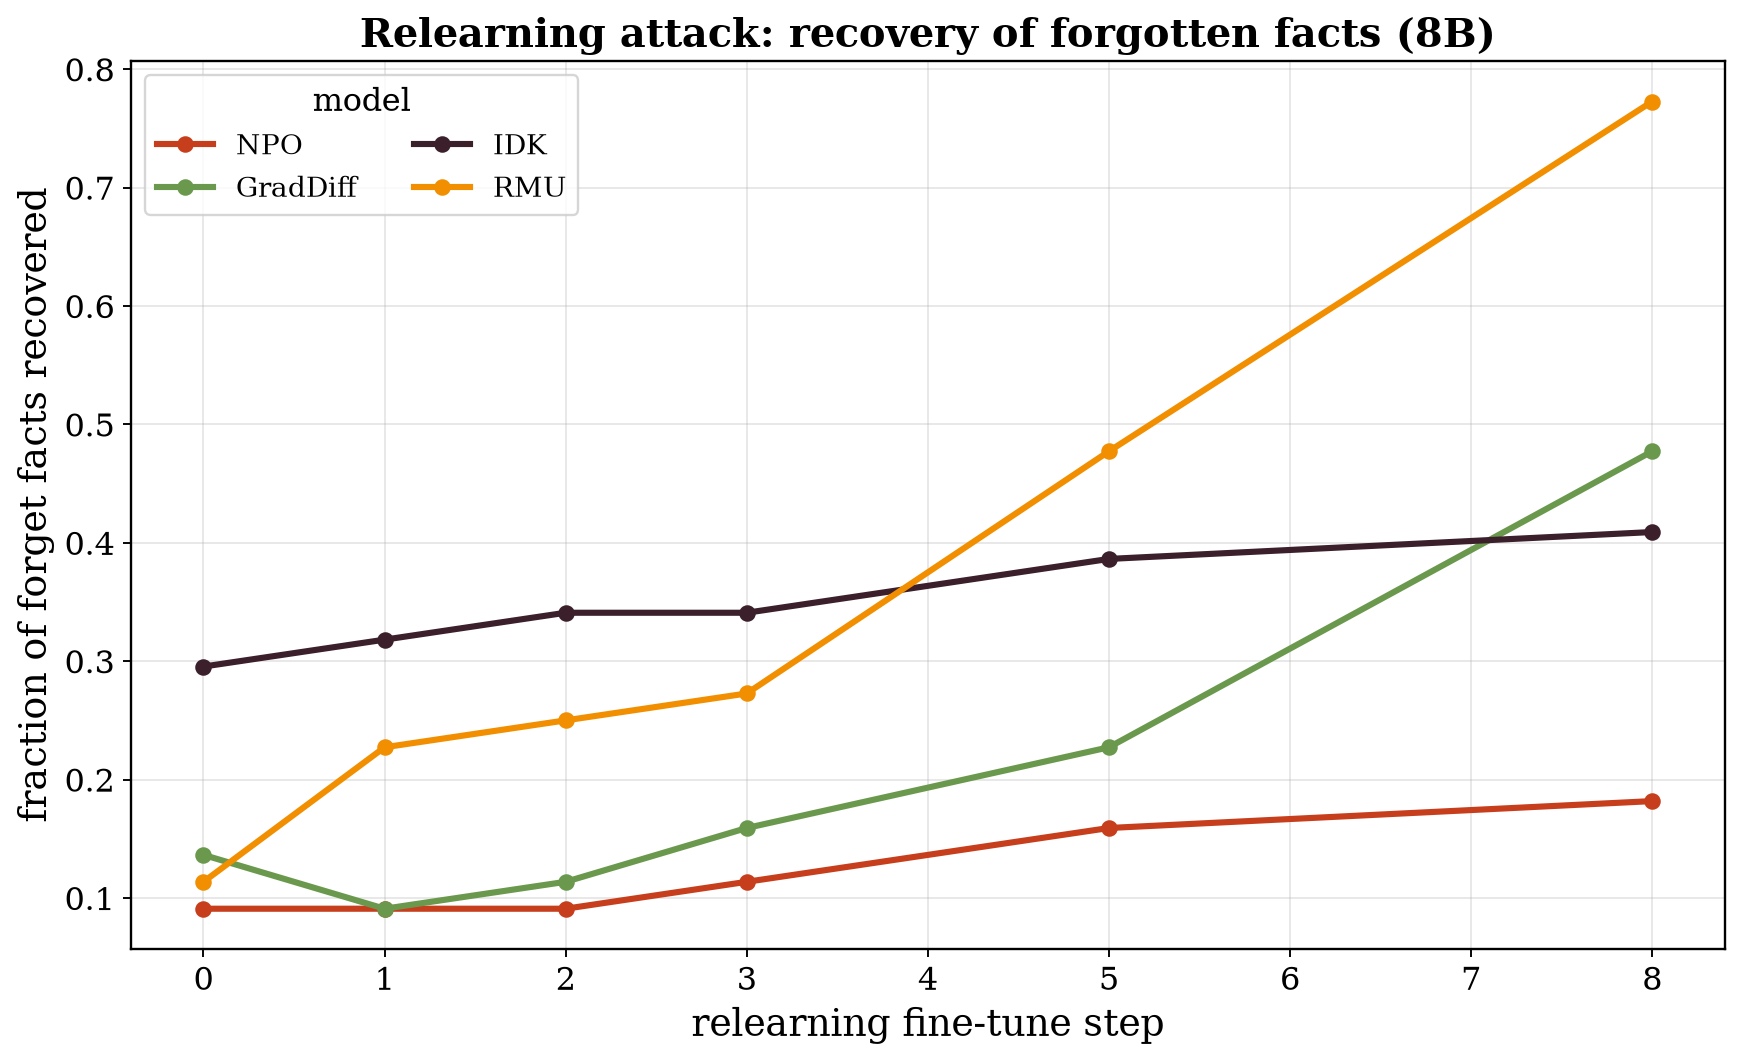
\includegraphics[width=0.7\textwidth]{relearn_recovery_8b}
  \caption[Relearning attack (8B)]{Relearning attack (8B). Fraction of forgotten facts recovered as the model is fine-tuned on the
  forget set. RMU, which buries the fact deepest, recovers fastest; IDK and NPO resist. The ordering is the
  inverse of mid-stack burial (Table~\ref{tab:midstack}).}
  \label{fig:relearn}
\end{figure}

\begin{figure}[t]
  \centering
  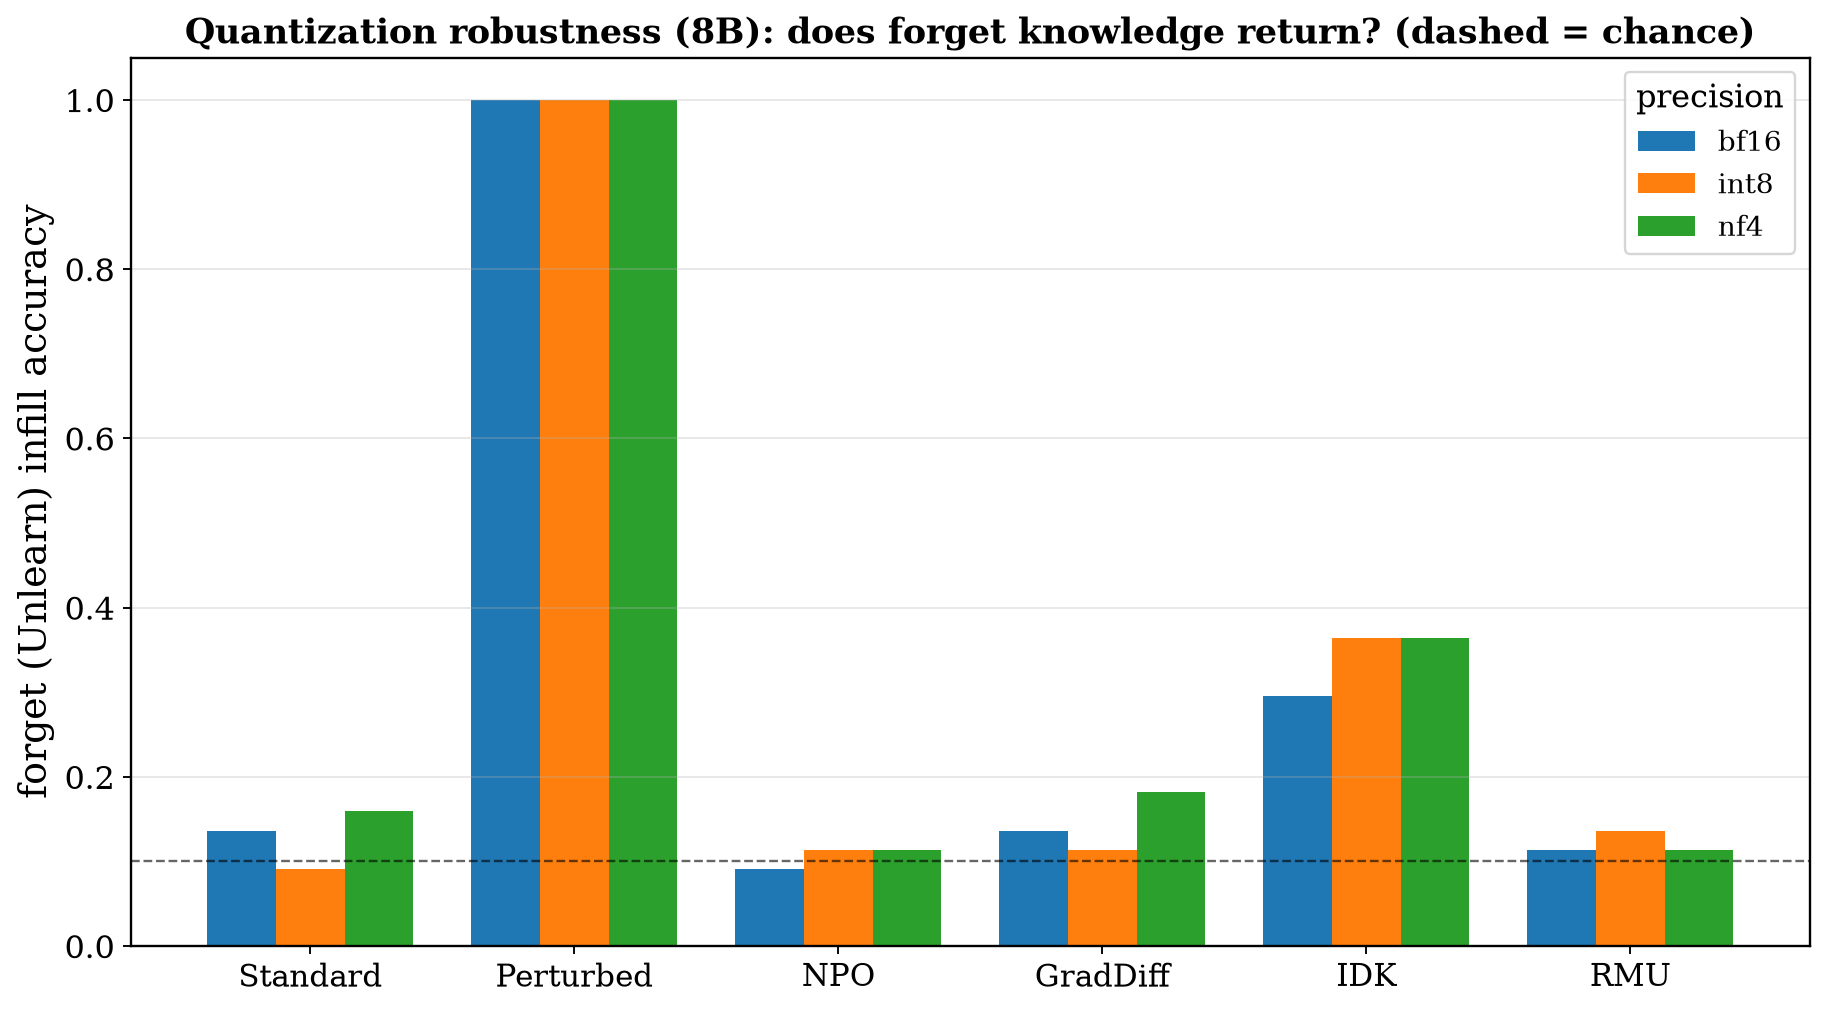
\includegraphics[width=0.8\textwidth]{quant_study_8b}
  \caption[Quantization robustness (8B)]{Quantization robustness (8B). Forget accuracy at bf16, int8, and 4-bit. Leakage is largest for
  the surface-level method IDK, matching the mechanistic taxonomy.}
  \label{fig:quant}
\end{figure}

\section{A Semantic-Residual Corroboration}
\label{sec:r-lsr}

Finally, an independent internal probe corroborates the taxonomy from a different angle. A semantic-residual
measure (the mass the model places on tokens semantically related to a held-out attribute, here
nationality) discriminates knowledge cleanly (Perturbed $\gg$ Standard, $p < 10^{-11}$ at both scales) and
orders the methods consistently with the birthdate analysis: NPO drives the semantic residual lowest, toward
the never-knew level (residual $0.11$ at 8B), IDK leaves it essentially intact ($1.00$, surface-level), and
GradDiff and RMU sit in between (Figure~\ref{fig:lsr}). Consistent with the calibrated wording used
throughout, we read this as the \emph{lowest measured semantic residual} for the nationality attribute, not
as proof of concept erasure. That two different internal probes, on two different attributes, agree on the
mechanism ordering is further evidence that the internal readout is tracking knowledge rather than an
artifact of any single measurement.

\begin{figure}[t]
  \centering
  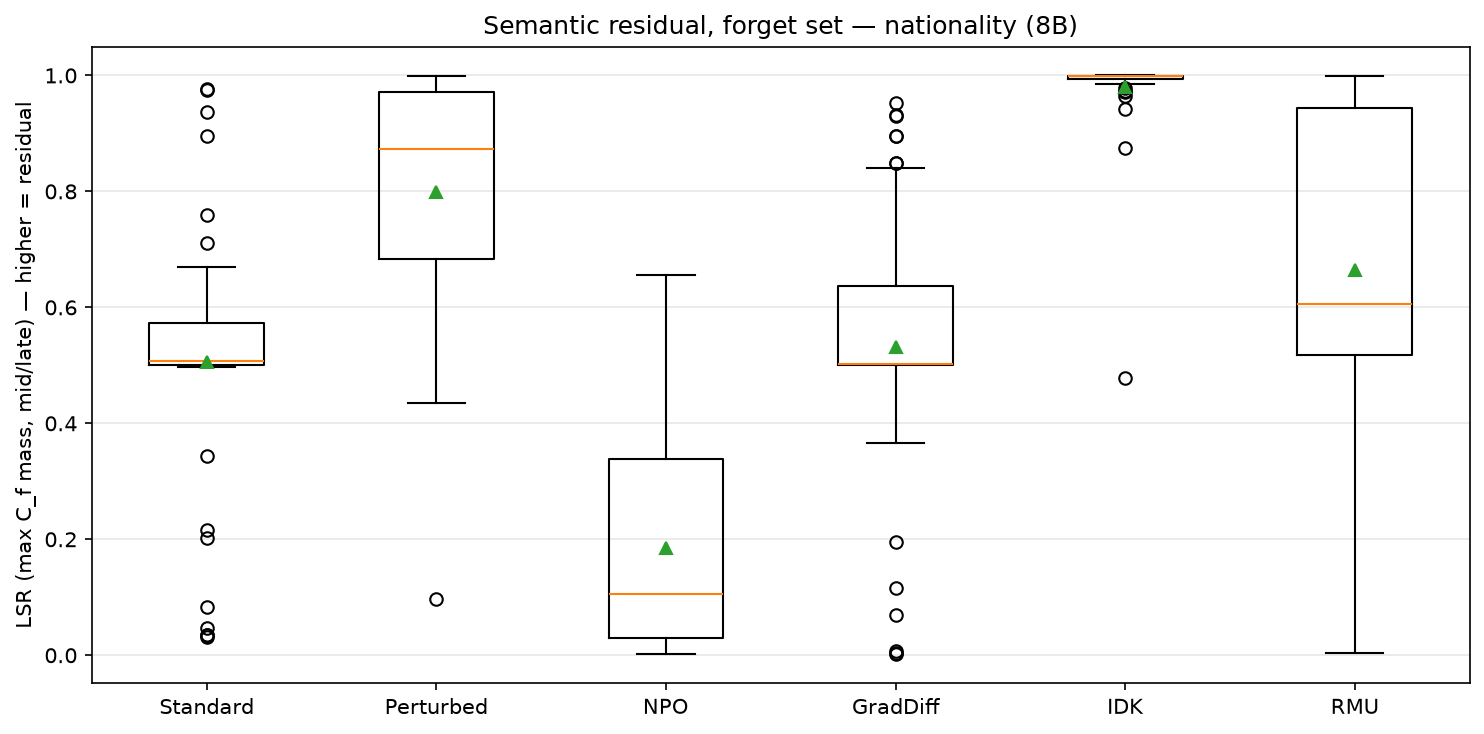
\includegraphics[width=0.7\textwidth]{lsr_boxplot_8b}
  \caption[Semantic-residual measure, nationality (8B)]{Semantic-residual measure on the nationality attribute (8B). It separates knows from never-knew
  and orders the methods as the birthdate analysis does (NPO drives the residual lowest, toward the
  never-knew level; IDK leaves it intact).}
  \label{fig:lsr}
\end{figure}

\section{Limitations}
\label{sec:r-limits}

We state the boundaries of these results honestly. The faithfulness meta-evaluation is run at 8B with
$n=44$ birthdate facts and a single fixed paraphrase and wrong-target realisation; the invariance ordering
is intrinsic to surface matching and the multi-paraphrase check supports it, but a design that samples many
rewordings would harden the claim. The faithfulness advantage is scale-dependent. At 1B, where the base
model memorises the facts only weakly, $D_\text{mech}$'s separation of knows from never-knew is
correspondingly weaker. A per-fact relearning route to validating the metric returned a null result (a
model-identity confound), so the faithfulness case rests on the meta-evaluation and the rank-by-layer story
rather than on predicting individual-fact recovery. Finally, the composite faithfulness score is a
convenience for ranking; the individual invariance and discrimination effect sizes are the primary
evidence.
